%
% $RCSfile: state_and_logic.tex,v $
%
% Copyright (C) 2002-2008. Christian Heller.
%
% Permission is granted to copy, distribute and/or modify this document
% under the terms of the GNU Free Documentation License, Version 1.1 or
% any later version published by the Free Software Foundation; with no
% Invariant Sections, with no Front-Cover Texts and with no Back-Cover
% Texts. A copy of the license is included in the section entitled
% "GNU Free Documentation License".
%
% http://www.cybop.net
% - Cybernetics Oriented Programming -
%
% http://www.resmedicinae.org
% - Information in Medicine -
%
% Version: $Revision: 1.1 $ $Date: 2008-08-19 20:41:09 $ $Author: christian $
% Authors: Christian Heller <christian.heller@tuxtax.de>
%

\chapter{State and Logic}
\label{state_and_logic_heading}
\index{State and Logic}
\index{Static Models}
\index{State Knowledge}
\index{Logic Knowledge}

\begin{flushright}
    \textsl{
        Time comes from a non-existent Future,\\
        into a non-durable Presence,\\
        and goes into a Past that has ceased to exist.
    }\\
    \textsc{Aurelius Augustinus}
\end{flushright}

\begin{wrapfigure}[6]{r}{4cm}
    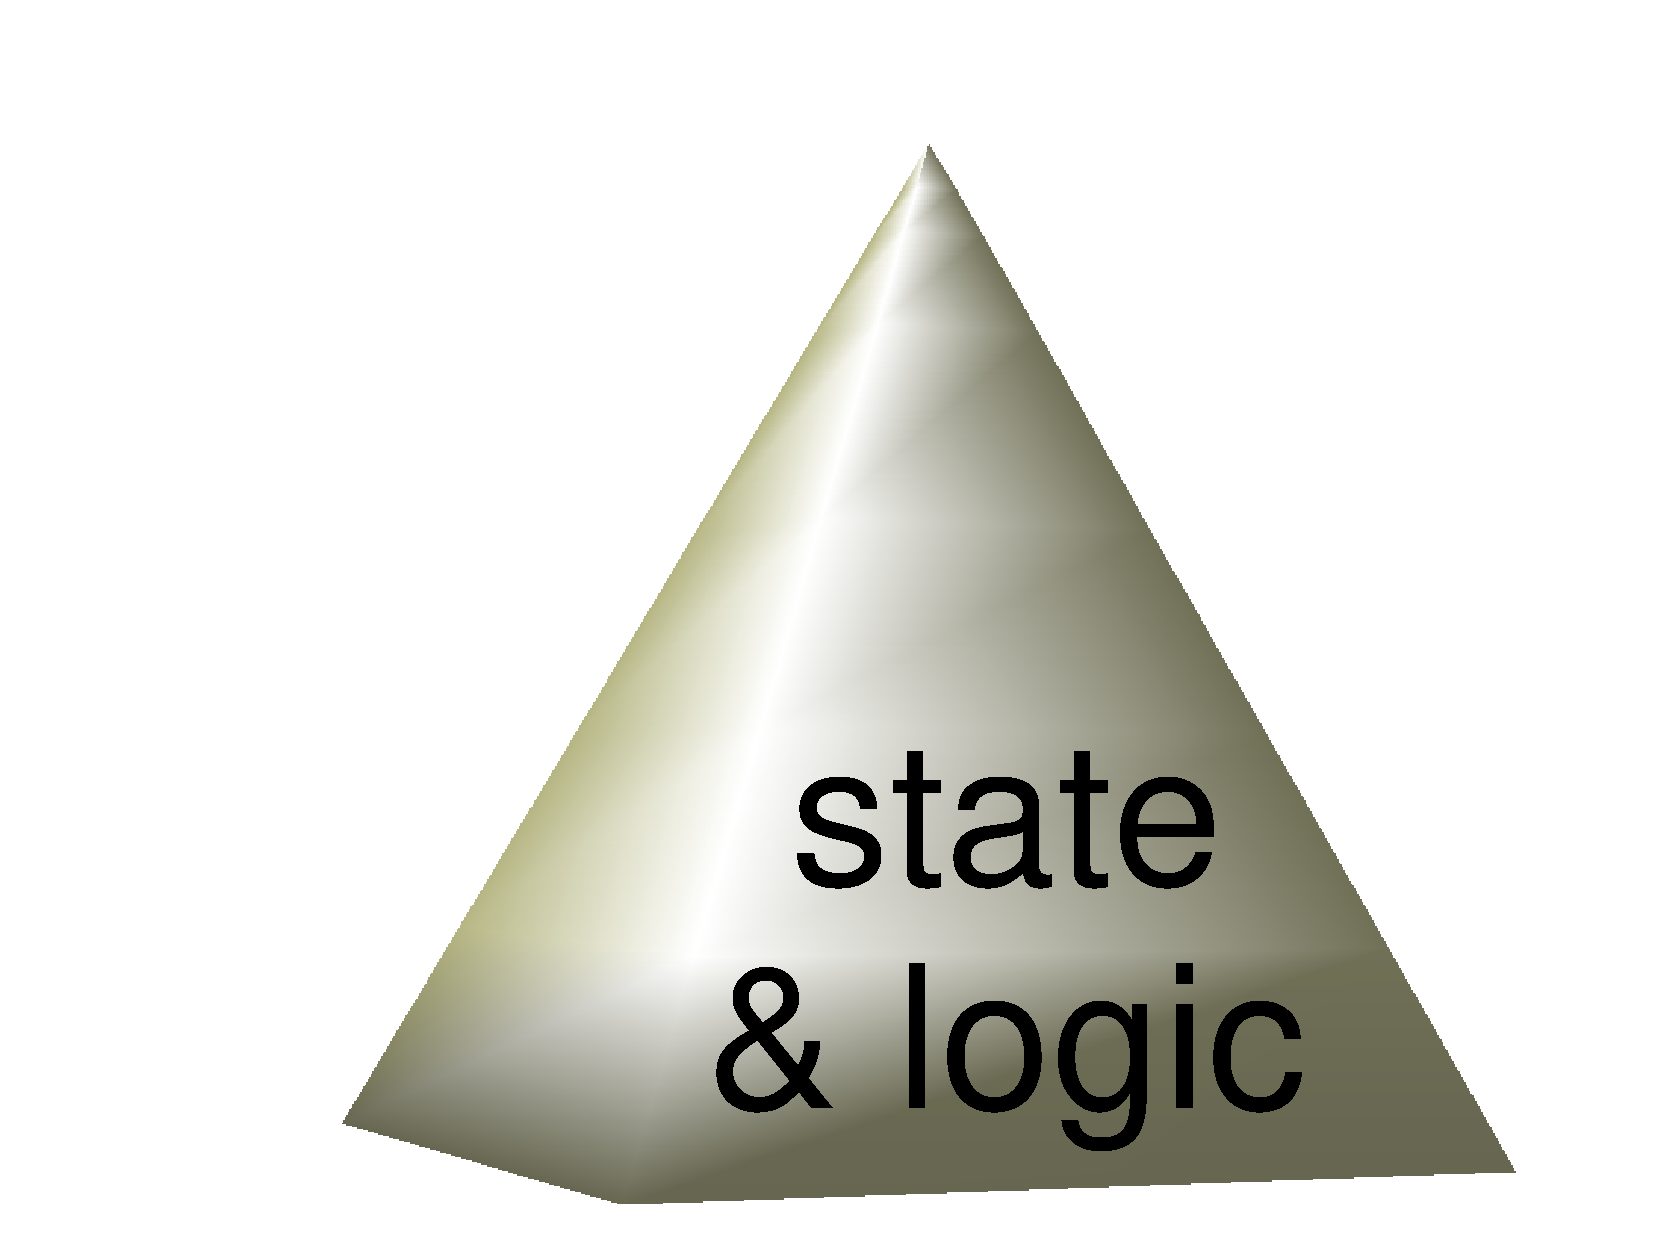
\includegraphics[scale=0.15,angle=-90]{graphic/contribution3.pdf}
\end{wrapfigure}

The previous two chapters justified a split of static knowledge from its
dynamic processing in a system, as well as the modelling of knowledge in a
double-hierarchy. This chapter, being the last of part
\ref{contribution_heading} of this work, elaborates on why it is important to
distinguish two different kinds of static models: \emph{State-} and
\emph{Logic Knowledge}.
\vspace{1cm}

%
% $RCSfile: a_changing_world.tex,v $
%
% Copyright (C) 2002-2008. Christian Heller.
%
% Permission is granted to copy, distribute and/or modify this document
% under the terms of the GNU Free Documentation License, Version 1.1 or
% any later version published by the Free Software Foundation; with no
% Invariant Sections, with no Front-Cover Texts and with no Back-Cover
% Texts. A copy of the license is included in the section entitled
% "GNU Free Documentation License".
%
% http://www.cybop.net
% - Cybernetics Oriented Programming -
%
% http://www.resmedicinae.org
% - Information in Medicine -
%
% Version: $Revision: 1.1 $ $Date: 2008-08-19 20:41:05 $ $Author: christian $
% Authors: Christian Heller <christian.heller@tuxtax.de>
%

\section{A Changing World}
\label{a_changing_world_heading}
\index{A Changing World}

To start with, this section looks into nature and several sciences once more,
to show how both kinds of knowledge (states and logic) appear in them.

%
% $RCSfile: change_follows_rules.tex,v $
%
% Copyright (C) 2002-2008. Christian Heller.
%
% Permission is granted to copy, distribute and/or modify this document
% under the terms of the GNU Free Documentation License, Version 1.1 or
% any later version published by the Free Software Foundation; with no
% Invariant Sections, with no Front-Cover Texts and with no Back-Cover
% Texts. A copy of the license is included in the section entitled
% "GNU Free Documentation License".
%
% http://www.cybop.net
% - Cybernetics Oriented Programming -
%
% http://www.resmedicinae.org
% - Information in Medicine -
%
% Version: $Revision: 1.1 $ $Date: 2008-08-19 20:41:05 $ $Author: christian $
% Authors: Christian Heller <christian.heller@tuxtax.de>
%

\subsection{Change follows Rules}
\label{change_follows_rules_heading}
\index{Change follows Rules}
\index{Motion}
\index{Flux}
\index{Activity}
\index{Rules}
\index{Logic}
\index{Inanimate World}
\index{Animate World}
\index{Nexus of Appearances}
\index{Chaos}
\index{Entropy}
\index{Repetition}
\index{Nesting}
\index{Randomness}
\index{Localised Structures}
\index{Universality}

What makes our world so interesting is not (only) its static structure, but its
permanent \emph{Change}. Already the ancient Greeks realised that \emph{Motion}
(\emph{Flux}/ \emph{Activity}/ \emph{Change}) is central to existence and
reality \cite{spaceandmotion}. Change happens according to \emph{Rules}
following a \emph{Logic}. John F. Sowa \cite[p. 132]{sowa} cites Immanuel Kant
who writes about the omnipresence of rules:

\begin{quote}
    Everything in nature, in the \emph{inanimate} as well as the \emph{animate}
    world, happens according to \emph{Rules}, although we do not always know
    these rules. Water falls according to the laws of gravity, and the locomotion
    of animals also takes place according to rules. The fish in the water, the
    bird in the air move according to rules. All nature actually is nothing but
    a \emph{Nexus} (inter-connection) of appearances according to rules; and
    there is nothing at all without rules. When we believe that we have come
    across an absence of rules, we can only say that the rules are unknown to us.
\end{quote}

Some people may believe that there are \emph{rule-less} things in universe, for
example kinds of \emph{Randomness} or \emph{Chaos} (with the \emph{Entropy}
used as a measure of the disorder present in a system \cite{wikipedia}).
Stephen Wolfram, however, demonstrated that everything in existence shows at
least one of the four following kinds of behaviour: \emph{Repetition},
\emph{Nesting}, \emph{Randomness}, \emph{Localised Structures}
(\emph{Universality}) (section \ref{basic_behaviour_heading}). And, he
reproduced these using simple rules encoded in abstract computer programs.

%
% $RCSfile: from_philosophy_to_mathematics.tex,v $
%
% Copyright (C) 2002-2008. Christian Heller.
%
% Permission is granted to copy, distribute and/or modify this document
% under the terms of the GNU Free Documentation License, Version 1.1 or
% any later version published by the Free Software Foundation; with no
% Invariant Sections, with no Front-Cover Texts and with no Back-Cover
% Texts. A copy of the license is included in the section entitled
% "GNU Free Documentation License".
%
% http://www.cybop.net
% - Cybernetics Oriented Programming -
%
% http://www.resmedicinae.org
% - Information in Medicine -
%
% Version: $Revision: 1.1 $ $Date: 2008-08-19 20:41:06 $ $Author: christian $
% Authors: Christian Heller <christian.heller@tuxtax.de>
%

\subsection{From Philosophy to Mathematics}
\label{from_philosophy_to_mathematics_heading}
\index{Philosophy and Mathematics}
\index{Logic}

Rules belong to a logic. Yet what is \emph{Logic} and how best to describe it
and the data it processes?

%
% $RCSfile: syllogism.tex,v $
%
% Copyright (C) 2002-2008. Christian Heller.
%
% Permission is granted to copy, distribute and/or modify this document
% under the terms of the GNU Free Documentation License, Version 1.1 or
% any later version published by the Free Software Foundation; with no
% Invariant Sections, with no Front-Cover Texts and with no Back-Cover
% Texts. A copy of the license is included in the section entitled
% "GNU Free Documentation License".
%
% http://www.cybop.net
% - Cybernetics Oriented Programming -
%
% http://www.resmedicinae.org
% - Information in Medicine -
%
% Version: $Revision: 1.1 $ $Date: 2008-08-19 20:41:09 $ $Author: christian $
% Authors: Christian Heller <christian.heller@tuxtax.de>
%

\subsubsection{Syllogism}
\label{syllogism_heading}
\index{Syllogism}
\index{Logic}
\index{Reasoning}
\index{Inference}
\index{Knowledge}
\index{Regress of Reasons}
\index{First Principles of Demonstration}
\index{Problem of First Principles}

Many descriptions exist for the term \emph{Logic}. \emph{Webster's Revised
Unabridged Dictionary} \cite{websters} defines it as:

\begin{quote}
    The science or art of exact reasoning, or of pure and formal thought, or of
    the laws according to which the processes of pure thinking should be conducted;
    the science of the formation and application of general notions; the science
    of generalization, judgment, classification, reasoning, and systematic
    arrangement; correct reasoning.
\end{quote}

The \emph{WordNet Dictionary} \cite{wordnet} calls it: \textit{A system of
reasoning.} A third definition given by the
\emph{Free On-line Dictionary of Computing} (FOLDOC) \cite{foldoc} shall be
mentioned: \textit{Logic is a branch of philosophy and mathematics that deals
with the formal principles, methods and criteria of validity of inference,
reasoning and knowledge.} \emph{The Devil's Dictionary} \cite{devils} means
that the basic of logic were the \emph{Syllogism}, consisting of three
propositions: a \emph{major} and a \emph{minor} \emph{Premise} (assumption) and
a \emph{Conclusion}. An example:

\begin{itemize}
    \item[-] \emph{Major Premise:} Sixty men can do a piece of work sixty times
        as quickly as one man.
    \item[-] \emph{Minor Premise:} One man can dig a post-hole in sixty seconds.
    \item[-] \emph{Conclusion:} Sixty men can dig a post-hole in one second.
\end{itemize}

The sense or nonsense (validity) of the results of reasoning is another issue.
\emph{Syllogism} means in short: \textit{to conclude by deductive reasoning; to
reckon all together; to bring at once before the mind; to infer}
\cite{websters}. What is important to note here is that logic describes the
laws after which one state (major and minor premise) is related to another
state (conclusion). It associates two statements and defines the rules for
deriving/ translating one from/ into the other.

As in all sciences, there is unsolved problems to \emph{Logic}, like the
\emph{Aristotelian Problem of First Principles}. Kelley L. Ross \cite{friesian}
writes:

\begin{quote}
    Logic is just the description of how (proposition) X implies (is a reason
    for) (proposition) Y and (proposition) Z, or that Y and Z are logical
    consequences of X. Logic can prove Y and Z on the basis of X, but it cannot
    prove X without further reasons (premises) \ldots\ If we continue to give
    reasons for reasons, from Z to Y, to X, to \ldots, this is called the
    \emph{Regress of Reasons}.
    Aristotle's second point, then, was just that the regress of reasons cannot
    be an infinite regress. If there is no end to our reasons for reasons, then
    nothing would ever be proven. We would just get tired of giving reasons,
    with nothing established any more securely than when we started. If there
    is to be no infinite regress, Aristotle realized, there must be propositions
    that do not need, for whatever reason, to be proven. Such propositions he
    called the first principles (archai, principii) of demonstration. How we
    would know first principles to be true, how we can verify them, if they
    cannot be proven is the \emph{Problem of First Principles}.
\end{quote}

This work does not attempt to further consider or even solve logical-
philosophical problems of that kind. Instead, it sticks with informatics which
deals with processing given states according to well-defined rules of logic and
focuses on their mathematical side, namely binary arithmetic and boolean logic,
as described following.

%
% $RCSfile: binary_arithmetic.tex,v $
%
% Copyright (C) 2002-2008. Christian Heller.
%
% Permission is granted to copy, distribute and/or modify this document
% under the terms of the GNU Free Documentation License, Version 1.1 or
% any later version published by the Free Software Foundation; with no
% Invariant Sections, with no Front-Cover Texts and with no Back-Cover
% Texts. A copy of the license is included in the section entitled
% "GNU Free Documentation License".
%
% http://www.cybop.net
% - Cybernetics Oriented Programming -
%
% http://www.resmedicinae.org
% - Information in Medicine -
%
% Version: $Revision: 1.1 $ $Date: 2008-08-19 20:41:05 $ $Author: christian $
% Authors: Christian Heller <christian.heller@tuxtax.de>
%

\subsubsection{Binary Arithmetic}
\label{binary_arithmetic_heading}
\index{Binary Arithmetic}
\index{Binary System of Arithmetic}
\index{Bit}
\index{Binary}
\index{Dialectic Dualism}
\index{Digital Technology}

One of the many great achievements of Gottfried Wilhelm Leibnitz (1646-1716)
\cite{standrews} was his development of the mathematical
\emph{Binary System of Arithmetic} (1679) \cite{friesian}. Unlike the
traditional number system that is based on the digits \emph{0..9}, the binary
system uses only two digits: \emph{0} and \emph{1}. Yet it is possible to
express any number as sequence of Bits (section \ref{digital_logic_heading}),
called a \emph{Binary}.

Many abstractions simplifying the real world are based on just \emph{two} views
(as investigated by the philosophical field of \emph{Dialectic Dualism}), for
example:

\begin{itemize}
    \item[-] Plus Infinity \& Minus Infinity (Mathematics)
    \item[-] Positive \& Negative (Physics)
    \item[-] Matter \& Antimatter (Physics)
    \item[-] Force \& Counterforce (Physics)
    \item[-] Masculine \& Feminine (Biology)
    \item[-] Active Neuron \& Passive Neuron (Neurology)
    \item[-] Black \& White (Psychology)
\end{itemize}

The binary system is now the basis of all digital technology. It enabled
scientists to construct simple electrical circuits and to combine them to
greater, more complicated ones and, finally, complex chips which are used in
every computer.

%
% $RCSfile: boolean_logic.tex,v $
%
% Copyright (c) 2002-2007. Christian Heller. All rights reserved.
%
% Permission is granted to copy, distribute and/or modify this document
% under the terms of the GNU Free Documentation License, Version 1.1 or
% any later version published by the Free Software Foundation; with no
% Invariant Sections, with no Front-Cover Texts and with no Back-Cover
% Texts. A copy of the license is included in the section entitled
% "GNU Free Documentation License".
%
% http://www.cybop.net
% - Cybernetics Oriented Programming -
%
% Version: $Revision: 1.1 $ $Date: 2007-07-17 20:02:36 $ $Author: christian $
% Authors: Christian Heller <christian.heller@tuxtax.de>
%

\section{Boolean Logic}
\label{boolean_logic_heading}
\index{Boolean Logic}

\input{not}
\input{neg}
\input{and}
\input{or}
\input{xor}


%
% $RCSfile: system.tex,v $
%
% Copyright (C) 2002-2008. Christian Heller.
%
% Permission is granted to copy, distribute and/or modify this document
% under the terms of the GNU Free Documentation License, Version 1.1 or
% any later version published by the Free Software Foundation; with no
% Invariant Sections, with no Front-Cover Texts and with no Back-Cover
% Texts. A copy of the license is included in the section entitled
% "GNU Free Documentation License".
%
% http://www.cybop.net
% - Cybernetics Oriented Programming -
%
% http://www.resmedicinae.org
% - Information in Medicine -
%
% Version: $Revision: 1.1 $ $Date: 2008-08-19 20:41:09 $ $Author: christian $
% Authors: Christian Heller <christian.heller@tuxtax.de>
%

\subsection{System}
\label{system_heading}
\index{System}
\index{Knowledge}
\index{Input of a System}
\index{Output of a System}
\index{Behaviour}

Earth is a system, a biotope and its biological creatures, including human
beings, are systems, our society, institutions, families and their individuals
are systems, machines and computers are systems -- and software applications
are systems. Actually, almost everything in existence can be treated and
simulated as system.

A rather general definition \cite{wikipedia} describes a system as: \textit{an
assemblage of inter-related elements comprising a unified whole.} Systems are
in a steady exchange with their environment. Information systems, for example,
exchange data. Depending on their structure, relations and contents, these may
be called \emph{Knowledge}. From the view of a system, the data are called
\emph{Input} and \emph{Output}. The output of one system can become the input
for another.

A certain logic with special rules can be abstracted in form of a \emph{System}.
The system's logic causes its characteristic \emph{Behaviour}, that is the way
its \emph{Input} gets manipulated to produce a specific \emph{Output}.

%
% $RCSfile: deterministic_and_stochastic_behaviour.tex,v $
%
% Copyright (C) 2002-2008. Christian Heller.
%
% Permission is granted to copy, distribute and/or modify this document
% under the terms of the GNU Free Documentation License, Version 1.1 or
% any later version published by the Free Software Foundation; with no
% Invariant Sections, with no Front-Cover Texts and with no Back-Cover
% Texts. A copy of the license is included in the section entitled
% "GNU Free Documentation License".
%
% http://www.cybop.net
% - Cybernetics Oriented Programming -
%
% http://www.resmedicinae.org
% - Information in Medicine -
%
% Version: $Revision: 1.1 $ $Date: 2008-08-19 20:41:06 $ $Author: christian $
% Authors: Christian Heller <christian.heller@tuxtax.de>
%

\subsubsection{Deterministic- and Stochastic Behaviour}
\label{deterministic_and_stochastic_behaviour_heading}
\index{Deterministic Behaviour}
\index{Stochastic Behaviour}
\index{Probabilistic Behaviour}
\index{Fuzzy Logic}
\index{Artificial Neural Network}
\index{ANN}

Systems can be distinguished by their behaviour, which can be \emph{deterministic}
or \emph{stochastic} (probabilistic). While the elements of the first work in a
predictable way, probabilistic systems are not fully transparent and their
results are only \emph{likely}, but never \emph{certain}. Living systems are
entirely probabilistic, because firstly, not all of their elements are known
and secondly, they always consist of sub systems on different functional
levels. \cite{sengbusch}

Two areas dealing with the simulation of stochastic behaviour are \emph{Fuzzy Logic}
%(section \ref{fuzzy_logic_heading})
and \emph{Artificial Neural Networks} (ANN).
%(section \ref{artificial_neural_network_heading}).
Most software systems
though, need \emph{reliable} (deterministic) behaviour delivering
\emph{predictable} results. Deterministic systems are therefore in the focus of
the research done in this work.

%
% $RCSfile: black_box.tex,v $
%
% Copyright (C) 2002-2008. Christian Heller.
%
% Permission is granted to copy, distribute and/or modify this document
% under the terms of the GNU Free Documentation License, Version 1.1 or
% any later version published by the Free Software Foundation; with no
% Invariant Sections, with no Front-Cover Texts and with no Back-Cover
% Texts. A copy of the license is included in the section entitled
% "GNU Free Documentation License".
%
% http://www.cybop.net
% - Cybernetics Oriented Programming -
%
% http://www.resmedicinae.org
% - Information in Medicine -
%
% Version: $Revision: 1.1 $ $Date: 2008-08-19 20:41:05 $ $Author: christian $
% Authors: Christian Heller <christian.heller@tuxtax.de>
%

\subsubsection{Black Box}
\label{black_box_heading}
\index{Black Box}
\index{Operation}
\index{Functional Elements}
\index{Complexity Hiding}
\index{Block Diagram}
\index{Unified Modeling Language}
\index{UML}

An \emph{Operation} can be well treated as system: it contains rules of logic
after which its input gets transformed into its output. But not all systems are
as easy as a simple operation; many are \emph{composed} of yet smaller systems.
Biological systems, for example, are extremely difficult to describe in their
entirety, with a simple mathematical formula.

A system may be seen as a number of interacting \emph{Functional Elements}. It
is these elements and their interactions which determine the specific
properties and behaviour of a system. However, for modelling the behaviour of a
transmission system, its inner structure is not important. Systems theory
focusses on the time-dependent progression of input- and output signals as well
as their relation.

A common technique in systems engineering is to reduce complexity by
\emph{hiding} functionality which is unimportant in the given context, inside a
system. One then talks of a system as \emph{Black Box} since only its input,
output and their relation, but not its inside, are considered (figure
\ref{blackbox_figure}). The black box provides an encapsulation towards the
infinite microcosm, and it knows nothing about its usage within a greater
macrocosm (section \ref{knowledge_ontology_heading}).

The usual way to illustrate system elements and their relations is the
\emph{Block Diagram}. It is an important instrument for system analysis. Many
structures and processes can be described in that manner. In software
engineering, the \emph{Unified Modeling Language} (UML) has become the de-facto
modelling standard instead.

%
% $RCSfile: open_and_closed_loop.tex,v $
%
% Copyright (C) 2002-2008. Christian Heller.
%
% Permission is granted to copy, distribute and/or modify this document
% under the terms of the GNU Free Documentation License, Version 1.1 or
% any later version published by the Free Software Foundation; with no
% Invariant Sections, with no Front-Cover Texts and with no Back-Cover
% Texts. A copy of the license is included in the section entitled
% "GNU Free Documentation License".
%
% http://www.cybop.net
% - Cybernetics Oriented Programming -
%
% http://www.resmedicinae.org
% - Information in Medicine -
%
% Version: $Revision: 1.1 $ $Date: 2008-08-19 20:41:08 $ $Author: christian $
% Authors: Christian Heller <christian.heller@tuxtax.de>
%

\subsubsection{Open- and Closed Loop}
\label{open_and_closed_loop_heading}
\index{Open Loop Control System}
\index{Closed Loop Control System}
\index{Automation Engineering}
\index{Control Engineering}
\index{Feedback Control System}
\index{Controller}
\index{Linear Behaviour}
\index{Proportional Behaviour}
\index{Differential Behaviour}
\index{Integral Behaviour}

The scientific discipline of \emph{Automation-} and \emph{Control Engineering}
knows two kinds of control systems: \emph{Open Loop} and \emph{Closed Loop}
(\emph{Feedback}). German language better confines both by defining the terms
\emph{Steuerung} (stearing) and \emph{Regelung} (controlling). Figure
\ref{blackbox_figure} illustrates a closed loop system, received by adding a
feedback loop to the black box mentioned before.

\begin{figure}[ht]
    \begin{center}
        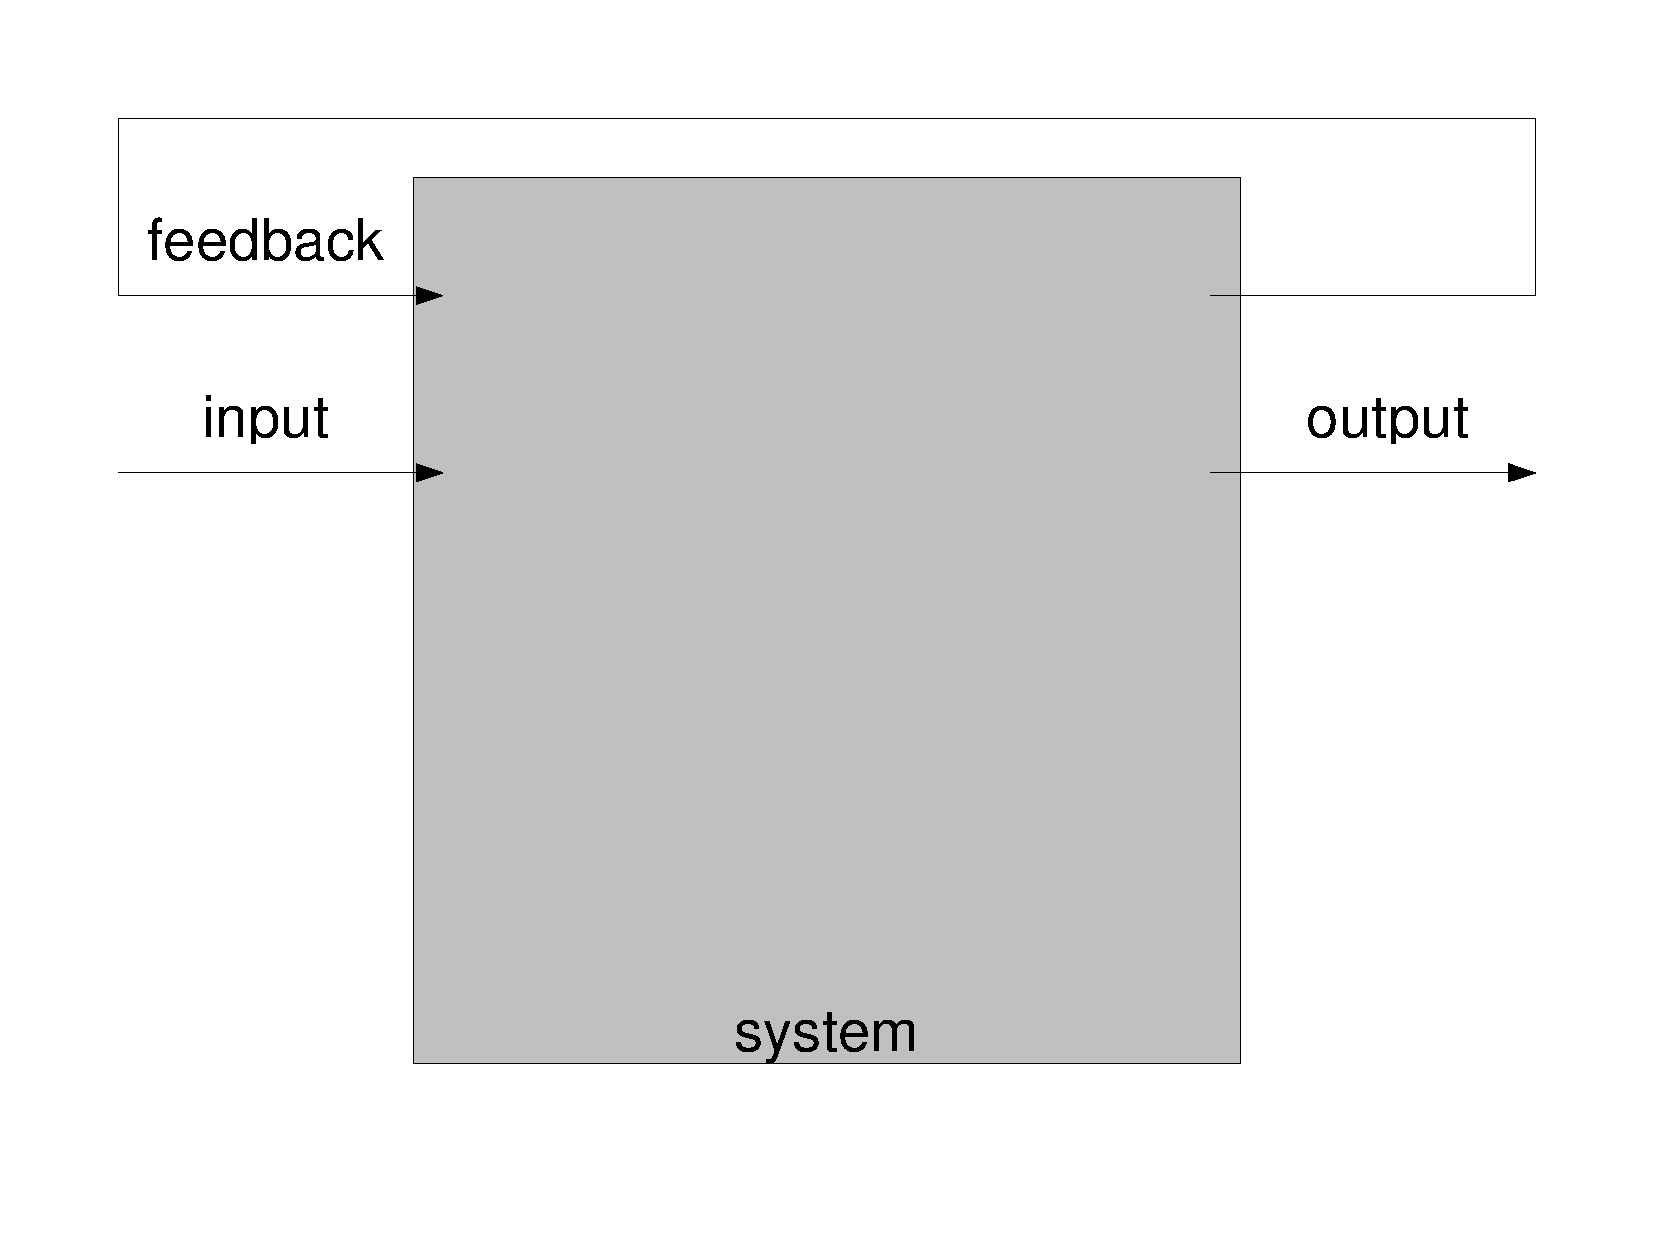
\includegraphics[scale=0.3,angle=-90]{graphic/blackbox.pdf}
        \caption{Closed Loop System with Feedback, modelled as Black Box}
        \label{blackbox_figure}
    \end{center}
\end{figure}

\newpage

A device controlling the behaviour of a system is called a \emph{Controller}.
Automation engineering uses electronic components such as \emph{Capacitor} and
\emph{Coil} to build controllers providing \emph{linear} (proportional),
\emph{differential} or \emph{integral} behaviour. In software engineering,
things are simpler. A computer program containing special mathematical
equations can simulate and control a system.

A software system's internal signal processing loop reads signals one by one,
from a signal memory (section \ref{knowledge_management_system_heading}).
While processing them, new signals may get created and placed in the signal
memory. This is how output results may be fed back to become a new input to the
software system.

%%
% $RCSfile: combinatoric_and_sequential_circuit.tex,v $
%
% Copyright (C) 2002-2008. Christian Heller.
%
% Permission is granted to copy, distribute and/or modify this document
% under the terms of the GNU Free Documentation License, Version 1.1 or
% any later version published by the Free Software Foundation; with no
% Invariant Sections, with no Front-Cover Texts and with no Back-Cover
% Texts. A copy of the license is included in the section entitled
% "GNU Free Documentation License".
%
% http://www.cybop.net
% - Cybernetics Oriented Programming -
%
% http://www.resmedicinae.org
% - Information in Medicine -
%
% Version: $Revision: 1.1 $ $Date: 2008-08-19 20:41:05 $ $Author: christian $
% Authors: Christian Heller <christian.heller@tuxtax.de>
%

\subsubsection{Combinatoric- and Sequential Circuit}
\label{combinatoric_and_sequential_circuit_heading}

\cite{wuttke}
Combinatoric Circuit (Stearing, Open Loop)
Sequential Circuit (Control, Closed Loop, Automat)
- internal state (output) is fed back to input
- necessary for conditions (if) in CYBOL
- a flag is set to true or false, as result of a comparison
- this flag is used as additional input to an operation which
only gets executed if the flag is true
- an input model for a CYBOL operation can represent an output model, at the same time;
similarly can an output represent an input (feedback loop);
the reference (path) to a knowledge model just has to be given as parameter of the operation;
it is up to the operation whether to use the referenced static model as input or output

%
% $RCSfile: input_output_and_rules.tex,v $
%
% Copyright (C) 2002-2008. Christian Heller.
%
% Permission is granted to copy, distribute and/or modify this document
% under the terms of the GNU Free Documentation License, Version 1.1 or
% any later version published by the Free Software Foundation; with no
% Invariant Sections, with no Front-Cover Texts and with no Back-Cover
% Texts. A copy of the license is included in the section entitled
% "GNU Free Documentation License".
%
% http://www.cybop.net
% - Cybernetics Oriented Programming -
%
% http://www.resmedicinae.org
% - Information in Medicine -
%
% Version: $Revision: 1.1 $ $Date: 2008-08-19 20:41:07 $ $Author: christian $
% Authors: Christian Heller <christian.heller@tuxtax.de>
%

\subsubsection{Input/Output and Rules}
\label{input_output_and_rules_heading}
\index{Data Structure}
\index{Enterprise Resource Planning System}
\index{ERP}
\index{Knowledge Model}
\index{Steady State}
\index{Converter containing Rules}
\index{Black Box}
\index{Logic Model}
\index{State Model}
\index{Information Flow}

In order to process data correctly, a system needs to know about their
\emph{Structure}. Software systems work with data belonging to some knowledge
model. Chapter \ref{knowledge_schema_heading} demonstrated how knowledge can be
modelled. Many applications keep their knowledge in special data files. Others,
such as \emph{Enterprise Resource Planning} (ERP) systems, retrieve their data
from a database. Even systems claiming to do nothing than pure data processing,
possibly using one operation only, rely on simple knowledge models, for at
least their \emph{Input/Output} (i/o) data.

Living systems rely on constantly exchanging information, energy, nutrients and
excretion products with their environment; they are never in a stationary, but
always in a \emph{Steady State}. A biological cell, for example, has inputs and
outputs and reacts in a certain manner which, after \cite{sengbusch}, is best
modelled with a \emph{Converter} containing \emph{Rules}, and treated as black
box. The cell's characteristic behaviour results from the way it relates inputs
to outputs.

\begin{figure}[ht]
    \begin{center}
        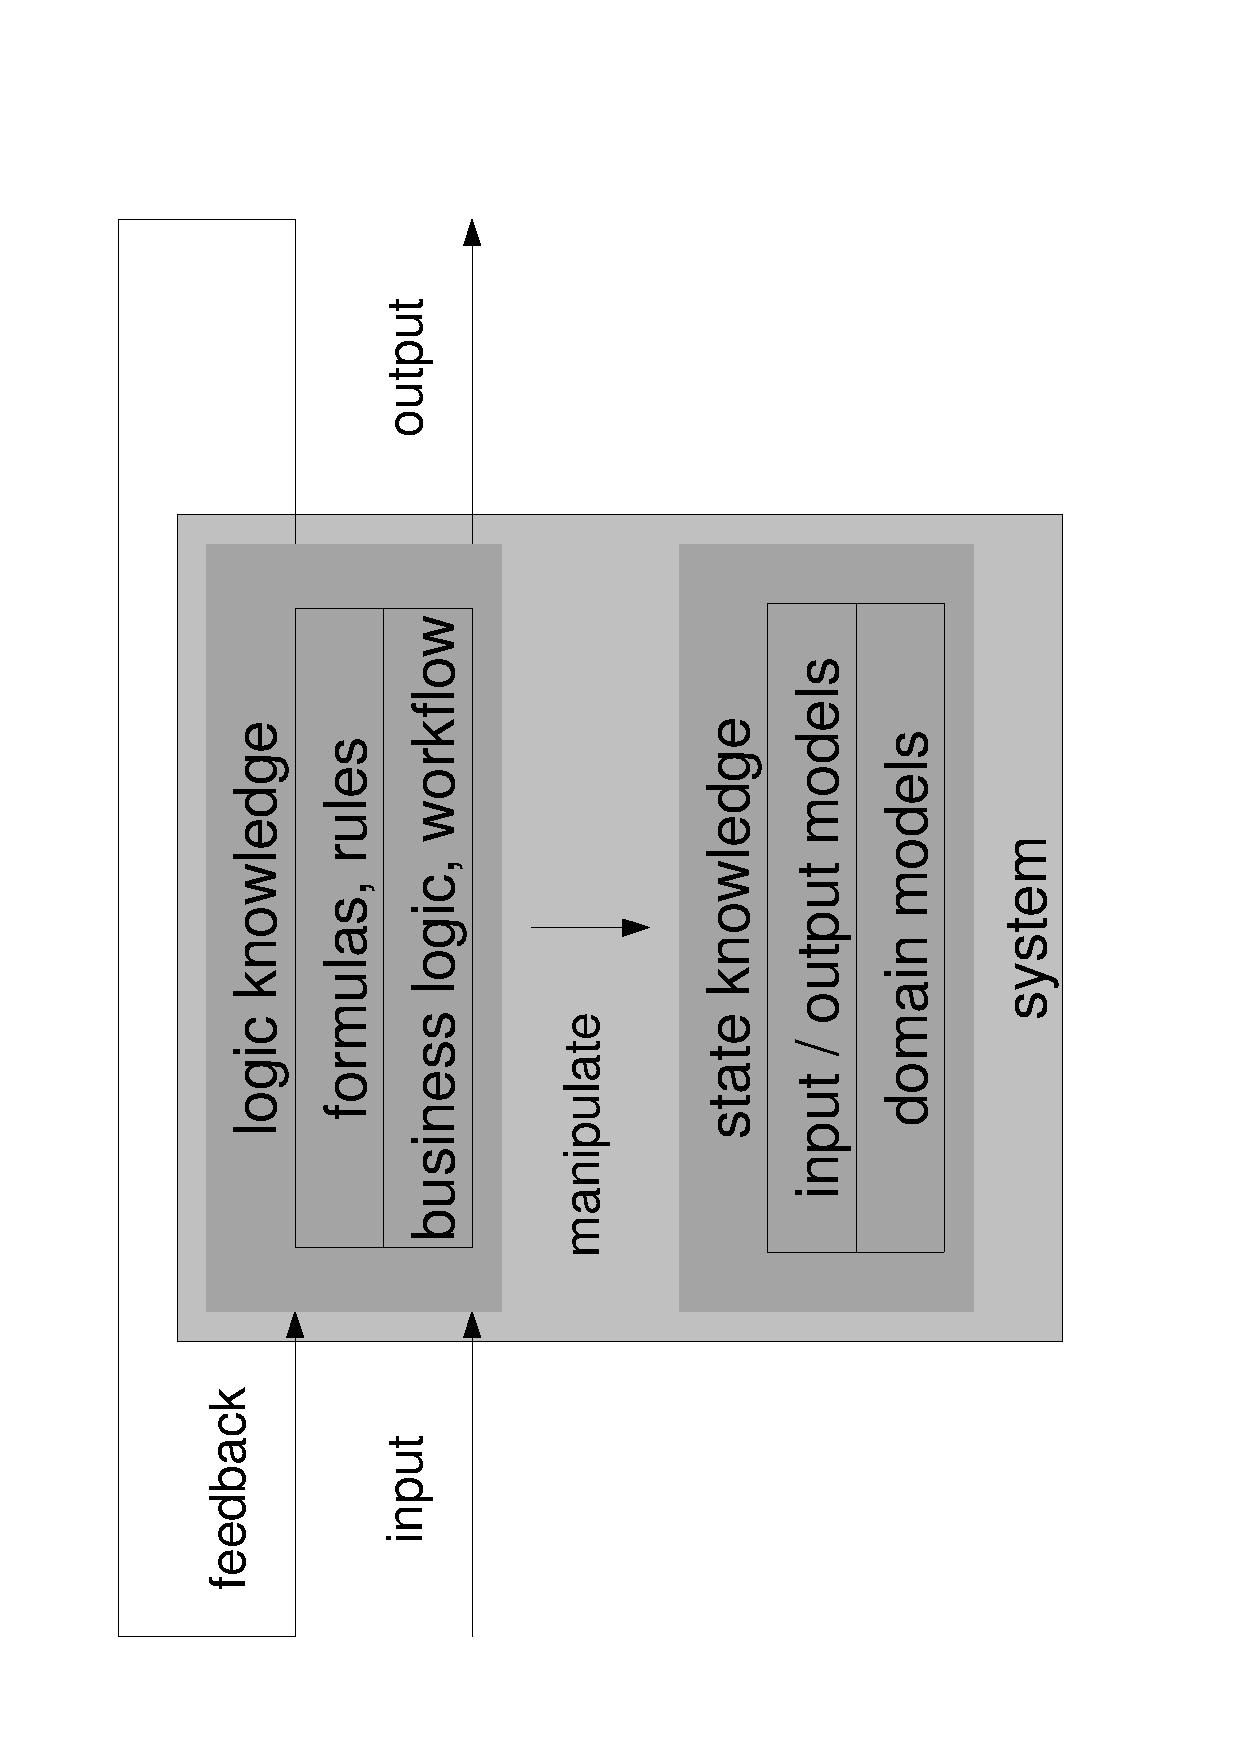
\includegraphics[scale=0.3,angle=-90]{graphic/manipulation.pdf}
        \caption{Logic translates between Input-, Domain- and Output States}
        \label{manipulation_figure}
    \end{center}
\end{figure}

Whilst figure \ref{blackbox_figure} illustrated the i/o flow of a system from
an \emph{outside} view, figure \ref{manipulation_figure} also considers the
state- and logic knowledge situated \emph{inside} a system. The arrow
indicating the information flow is directed from \emph{Logic-} towards
\emph{State} models, because the former manipulate the latter.


%
% $RCSfile: self_awareness.tex,v $
%
% Copyright (C) 2002-2008. Christian Heller.
%
% Permission is granted to copy, distribute and/or modify this document
% under the terms of the GNU Free Documentation License, Version 1.1 or
% any later version published by the Free Software Foundation; with no
% Invariant Sections, with no Front-Cover Texts and with no Back-Cover
% Texts. A copy of the license is included in the section entitled
% "GNU Free Documentation License".
%
% http://www.cybop.net
% - Cybernetics Oriented Programming -
%
% http://www.resmedicinae.org
% - Information in Medicine -
%
% Version: $Revision: 1.1 $ $Date: 2008-08-19 20:41:08 $ $Author: christian $
% Authors: Christian Heller <christian.heller@tuxtax.de>
%

\subsection{Self Awareness}
\label{self_awareness_heading}
\index{Self Awareness}
\index{Mind}
\index{Brain}
\index{Vegetative Nerve System}
\index{Animalic Nerve System}
\index{Agent}
\index{Agent Oriented Programming}
\index{AGOP}
\index{Capabilities of an Agent}
\index{Mental State of an Agent}

One of the particular characteristics of human beings is their ability for
\emph{Self Awareness}. It contrasts the human- with an animal mind because it
permits humans not only to understand what is going on in their environment,
but also themselves and their being in this world. In other words, the
\emph{Mind} knows about itself and about its existence in form of the human
organ called \emph{Brain}, as its physical carrier and as the place of
thinking.

Of course, the mind also knows about further organs and body parts. Some of the
concepts stored in it contain the characteristics of a human being. This
knowledge of the structure of the human body is necessary for the mind to be
able to steer it. While the functions for living are \emph{passively}
controlled by the \emph{vegetative} (unconscious) nerve system, sensoric and
motoric (input/ output) organs need to be controlled \emph{actively}, by the
\emph{animalic} (conscious) nerve system.

A system also needs to know about its own abilities, in order to be able to
communicate. It has to have a concept of its communication organs/ devices,
spoken languages etc. This counts for a human- as for a computer system. The
\emph{Agent} systems used in \emph{Agent Oriented Programming} (AGOP) (section
\ref{agent_oriented_programming_heading}) know about their \emph{Capabilities},
which are stored together with other knowledge as their \emph{Mental State}.

%
% $RCSfile: human_body.tex,v $
%
% Copyright (C) 2002-2008. Christian Heller.
%
% Permission is granted to copy, distribute and/or modify this document
% under the terms of the GNU Free Documentation License, Version 1.1 or
% any later version published by the Free Software Foundation; with no
% Invariant Sections, with no Front-Cover Texts and with no Back-Cover
% Texts. A copy of the license is included in the section entitled
% "GNU Free Documentation License".
%
% http://www.cybop.net
% - Cybernetics Oriented Programming -
%
% http://www.resmedicinae.org
% - Information in Medicine -
%
% Version: $Revision: 1.1 $ $Date: 2008-08-19 20:41:07 $ $Author: christian $
% Authors: Christian Heller <christian.heller@tuxtax.de>
%

\subsubsection{Human Body}
\label{human_body_heading}
\index{Human Body}
\index{Sensoric Organs}
\index{Motoric Organs}
\index{Human Senses}
\index{Nerve Cell}
\index{Muscle Cell}
\index{Information Reception}
\index{Information Sending}

Figure \ref{human_figure} shows parts of the animalic nerve system of a human
being. \emph{Sensoric} organs are used for information input; \emph{motoric}
organs for information output.

\begin{figure}[ht]
    \begin{center}
        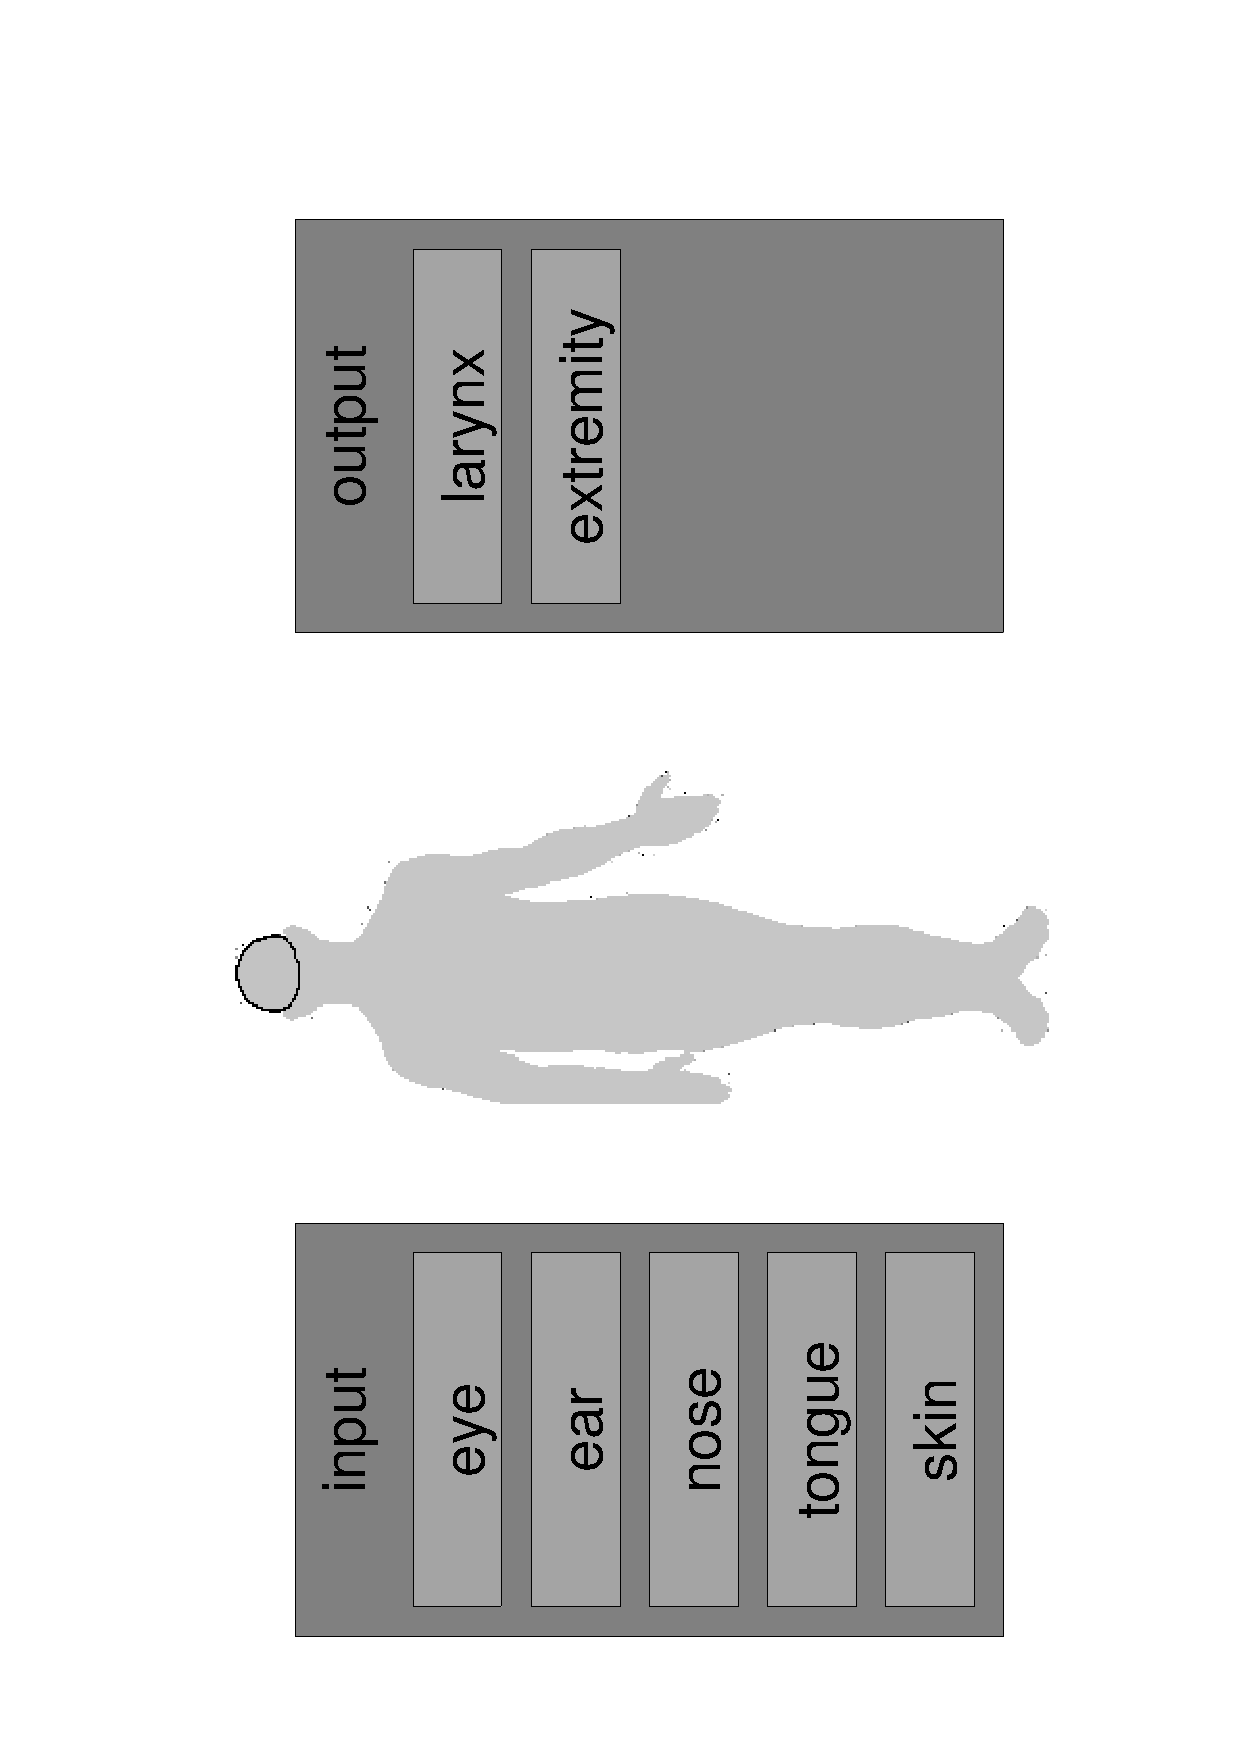
\includegraphics[scale=0.3,angle=-90]{graphic/human.pdf}
        \caption{Human Body with Sensoric and Motoric Organs}
        \label{human_figure}
    \end{center}
\end{figure}

The five (seven) human senses were already shown in table \ref{senses_table}.
They are able to receive signals which are transported by different mediums.
The transport mechanisms rely on various physical and chemical \emph{Effects},
as shown in table \ref{effects_table}. Each sense is represented by an
\emph{Organ}. The optic cells of the retina of an \emph{Eye} bundle light
stimuli which the optic nerve forwards as electrical signal to the brain. The
inner \emph{Ear} transforms oscillation frequencies of sound-waves into
electrical signals to send on to the brain. And so forth.

\begin{table}[ht]
    \begin{center}
        \begin{footnotesize}
        \begin{tabular}{| p{30mm} | p{50mm} | p{25mm} |}
            \hline
            \textbf{Effect} & \textbf{Science} & \textbf{Sense}\\
            \hline
            Oscillation, Wave & Physics, Mechanics & Seeing, Hearing\\
            \hline
            Density, Temperature & Physics, Mechanics, Thermodynamics & Tactile\\
            \hline
            Aroma & Chemistry & Smelling, Tasting\\
            \hline
        \end{tabular}
        \end{footnotesize}
        \caption{Effects as Basis of Sensing}
        \label{effects_table}
    \end{center}
\end{table}

While the \emph{Reception} of information is based on \emph{Nerve Cells}, it is
\emph{Muscle Cells} which are responsible for information \emph{Sending}.
Humans communicate for example through visual \emph{Gestures} using their
\emph{Extremities} or through acoustical \emph{Talking} using their
\emph{Larynx}/ \emph{Vocal Chords}. The latter, too, is based on muscle
activity.

%
% $RCSfile: computer_hardware.tex,v $
%
% Copyright (C) 2002-2008. Christian Heller.
%
% Permission is granted to copy, distribute and/or modify this document
% under the terms of the GNU Free Documentation License, Version 1.1 or
% any later version published by the Free Software Foundation; with no
% Invariant Sections, with no Front-Cover Texts and with no Back-Cover
% Texts. A copy of the license is included in the section entitled
% "GNU Free Documentation License".
%
% http://www.cybop.net
% - Cybernetics Oriented Programming -
%
% http://www.resmedicinae.org
% - Information in Medicine -
%
% Version: $Revision: 1.1 $ $Date: 2008-08-19 20:41:06 $ $Author: christian $
% Authors: Christian Heller <christian.heller@tuxtax.de>
%

\subsubsection{Computer Hardware}
\label{computer_hardware_heading}
\index{Computer Hardware}
\index{Human Being}
\index{Technical Environment}
\index{Biological Environment}

Gilbert Carl Herschberger II writes \cite{josgeneral}: \textit{A computer is a
grossly oversimplified model of a human being. Humans can learn more about
themselves by working with this model. And, they might learn more about what
makes a good model by looking at themselves.} To the many analogies a computer
has with a human being belong its input/ output (i/o) devices (figure
\ref{computer_figure}), many of which have an equivalent organ in the human
body:

\begin{itemize}
    \item[-] \emph{Eye}: Camera, Scanner
    \item[-] \emph{Ear}: Microphone
    \item[-] \emph{Nose, Tongue}: Sensors
    \item[-] \emph{Skin}: Keyboard, Mouse, Joystick
    \item[-] \emph{Larynx}: Loudspeaker
    \item[-] \emph{Extremity}: Monitor, Printer, Braille Panel, Arm, Wheel
\end{itemize}

\begin{figure}[ht]
    \begin{center}
        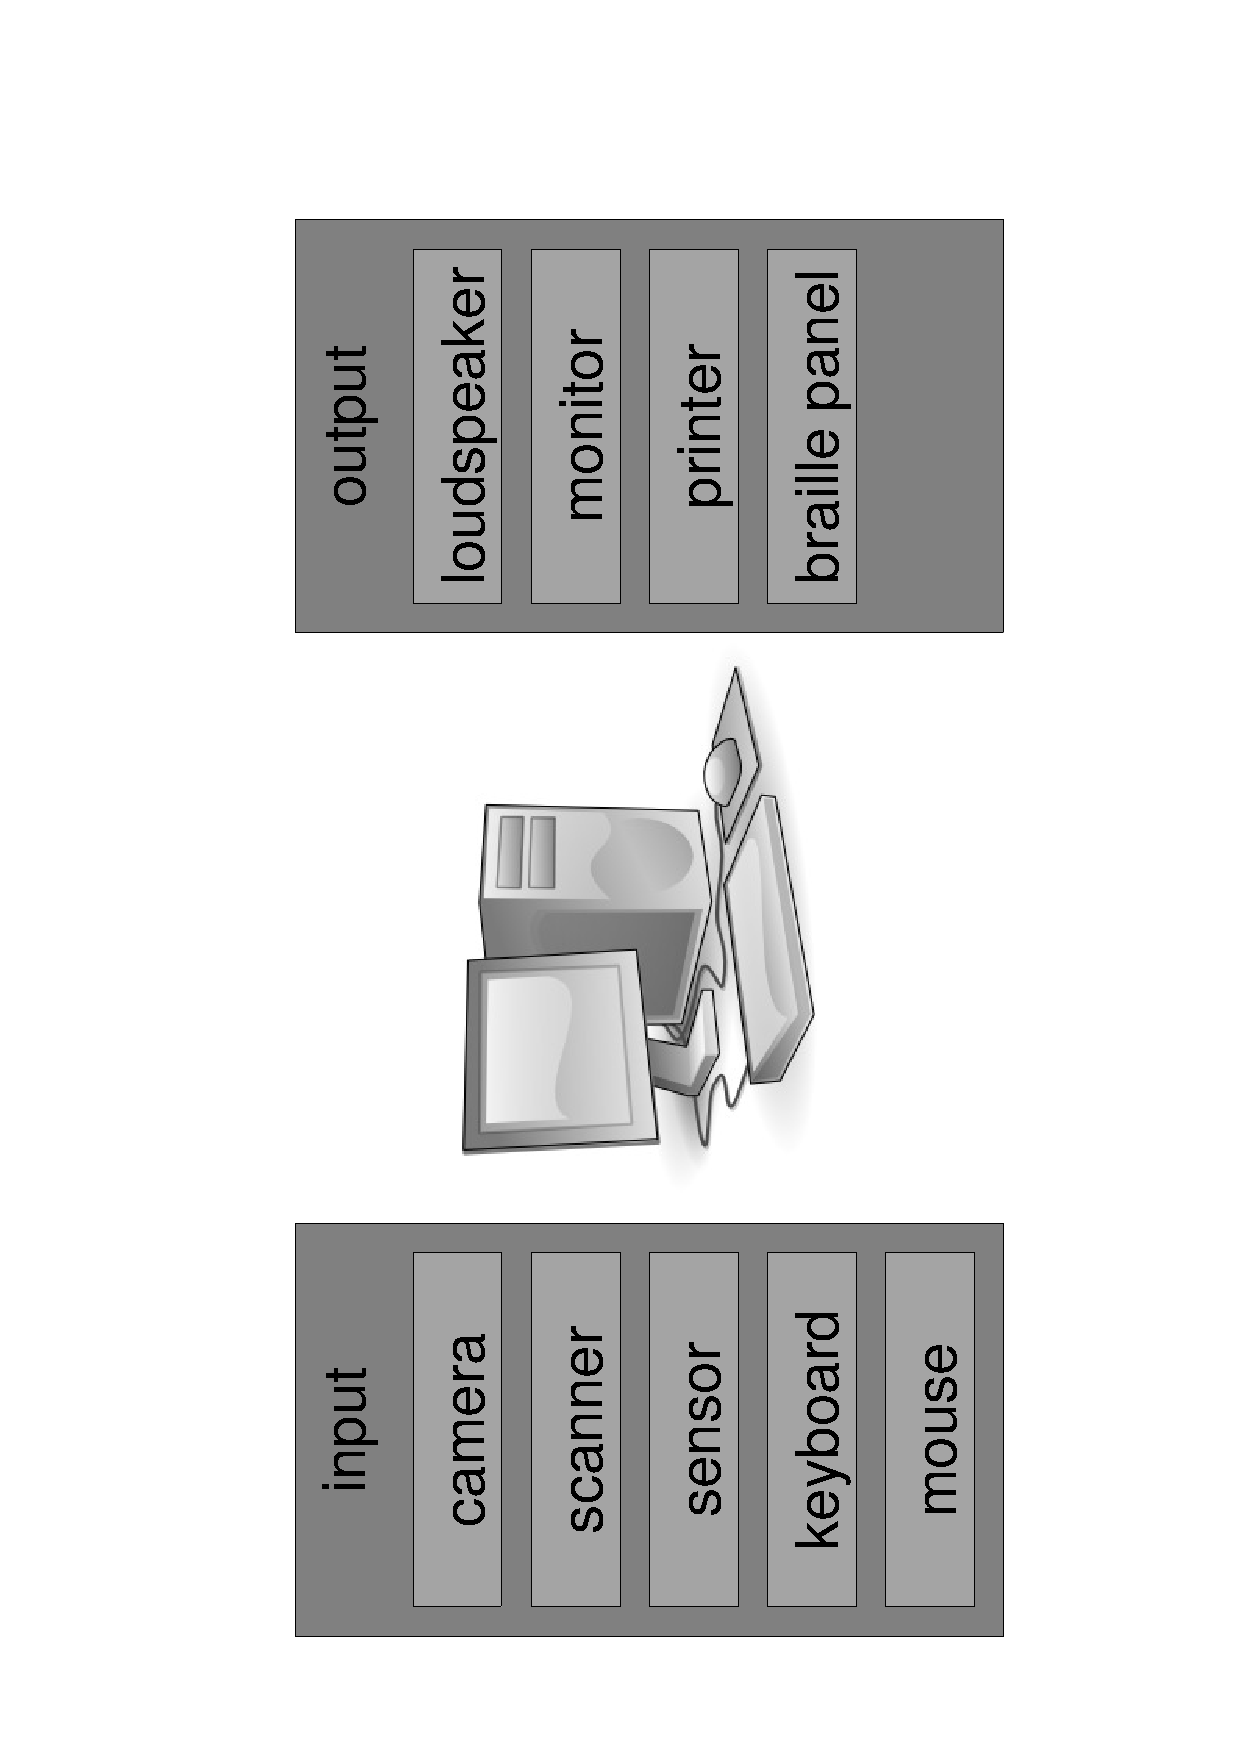
\includegraphics[scale=0.3,angle=-90]{graphic/computer.pdf}
        \caption{Computer Hardware with Input- and Output Devices}
        \label{computer_figure}
    \end{center}
\end{figure}

The difference to \emph{Robotics} is that a robot has additional devices.
Various \emph{Sensors} are used for information input; many moveable parts like
\emph{Arms} or \emph{Wheels} take motoric action and can be compared to the
extremities of the human body. Table \ref{environment_table} gives an
impression of how technical and biological environments can be compared.

\begin{figure}[ht]
    \begin{center}
        \begin{footnotesize}
        \begin{tabular}{| p{25mm} | p{50mm} | p{30mm} |}
            \hline
            \textbf{Ontological Level} & \textbf{Technical System} & \textbf{Biological Equivalent}\\
            \hline
            Network & Internet, Wide Area Network (WAN) & Society, Biotope\\
            \hline
            Family & Local Area Network (LAN) & Family\\
            \hline
            System & Computer & Organism\\
            \hline
            Block & Component & Organ\\
            \hline
        \end{tabular}
        \end{footnotesize}
        \caption{Ontology comparing Technical- and Biological Environment}
        \label{environment_table}
    \end{center}
\end{figure}

To sum up: Among the abstract knowledge models stored in a system are some that
describe the structure and capabilities of the system itself.


%
% $RCSfile: communication.tex,v $
%
% Copyright (c) 2002-2007. Christian Heller. All rights reserved.
%
% Permission is granted to copy, distribute and/or modify this document
% under the terms of the GNU Free Documentation License, Version 1.1 or
% any later version published by the Free Software Foundation; with no
% Invariant Sections, with no Front-Cover Texts and with no Back-Cover
% Texts. A copy of the license is included in the section entitled
% "GNU Free Documentation License".
%
% http://www.cybop.net
% - Cybernetics Oriented Programming -
%
% Version: $Revision: 1.2 $ $Date: 2007-08-01 13:59:00 $ $Author: christian $
% Authors: Christian Heller <christian.heller@tuxtax.de>
%

\section{Communication}
\label{communication_heading}
\index{Communication}

%
% $RCSfile: send.tex,v $
%
% Copyright (c) 2002-2007. Christian Heller. All rights reserved.
%
% Permission is granted to copy, distribute and/or modify this document
% under the terms of the GNU Free Documentation License, Version 1.1 or
% any later version published by the Free Software Foundation; with no
% Invariant Sections, with no Front-Cover Texts and with no Back-Cover
% Texts. A copy of the license is included in the section entitled
% "GNU Free Documentation License".
%
% http://www.cybop.net
% - Cybernetics Oriented Programming -
%
% Version: $Revision: 1.1 $ $Date: 2007-07-17 20:02:36 $ $Author: christian $
% Authors: Christian Heller <christian.heller@tuxtax.de>
%

\subsection{Send}
\label{send_heading}
\index{Send}

This operation is able to send a message via textual, graphical or web user
interface, or to the file system or also as shell output directly.

\subsubsection{Channel Property}

\emph{required}

name=\texttt{'channel'}\\
abstraction=\texttt{'character'}\\
model=\texttt{'inline' \vline\ 'file'}

The channel via which to send the message.

\subsubsection{Language Property}

\emph{required}

name=\texttt{'language'}\\
abstraction=\texttt{'character'}\\
model=\texttt{'tui' \vline\ 'gui' \vline\ 'wui' \vline\ 'file' \vline\ 'shell' \vline\ etc.}

The language into which to encode the message before sending it.

\subsubsection{Mode Property}

\emph{required}

name=\texttt{'mode'}\\
abstraction=\texttt{'character'}\\
model=\texttt{'client' \vline\ 'server'}

The mode of communication.

\subsubsection{Namespace Property}

\emph{required}

name=\texttt{'namespace'}\\
abstraction=\texttt{'character'}\\
model=\texttt{'local' \vline\ 'inet' \vline\ 'inet6' \vline\ 'ns' \vline\ 'iso' \vline\ 'ccitt' \vline\ 'implink' \vline\ 'route'}

The namespace of the socket.

\subsubsection{Style Property}

\emph{required}

name=\texttt{'style'}\\
abstraction=\texttt{'character'}\\
model=\texttt{'stream' \vline\ 'datagram' \vline\ 'raw'}

The style of communication.

\subsubsection{Sender Property}

\emph{required}

name=\texttt{'sender'}\\
abstraction=\texttt{'character'}\\
model=\texttt{name of sending system}

The name of the system sending the message.

\subsubsection{Receiver Property}

\emph{required}

name=\texttt{'receiver'}\\
abstraction=\texttt{'character'}\\
model=\texttt{name of receiving system}

The name of the system receiving the message.

\subsubsection{Message Property}

\emph{required}

name=\texttt{'message'}\\
abstraction=\texttt{'knowledge' \vline\ 'encapsulated'}\\
model=\texttt{message knowledge model path}

The actual message to be sent to another system.

\subsubsection{Area Property}

\emph{optional}

name=\texttt{'area'}\\
abstraction=\texttt{'knowledge' \vline\ 'encapsulated'}\\
model=\texttt{knowledge path to part model to be repainted}

The user interface area to be repainted. It is normally just a part of the
whole user interface model. This property helps to speed up repainting while
avoiding user interface flickering.

\subsubsection{Clean Property}

\emph{optional}

name=\texttt{'clean'}\\
abstraction=\texttt{'boolean'}\\
model=\texttt{'true' \vline\ 'false'}

This property indicates whether or not to clear the screen before painting a
user interface.

\subsubsection{New Line Property}

\emph{optional}

name=\texttt{'new\_line'}\\
abstraction=\texttt{'boolean'}\\
model=\texttt{'true' \vline\ 'false'}

This property indicates whether or not to add a new line after having printed
the message on screen.

%
% $RCSfile: receive.tex,v $
%
% Copyright (c) 2002-2007. Christian Heller. All rights reserved.
%
% Permission is granted to copy, distribute and/or modify this document
% under the terms of the GNU Free Documentation License, Version 1.1 or
% any later version published by the Free Software Foundation; with no
% Invariant Sections, with no Front-Cover Texts and with no Back-Cover
% Texts. A copy of the license is included in the section entitled
% "GNU Free Documentation License".
%
% http://www.cybop.net
% - Cybernetics Oriented Programming -
%
% Version: $Revision: 1.2 $ $Date: 2007-08-01 13:59:00 $ $Author: christian $
% Authors: Christian Heller <christian.heller@tuxtax.de>
%

\subsection{Receive}
\label{receive_heading}
\index{Receive}

This operation receives data from the given data source.

\subsubsection{Example}

\begin{scriptsize}
    \begin{verbatim}
<part name="receive_patients" channel="inline" abstraction="operation" model="receive">
    <property name="channel" channel="inline" abstraction="character" model="file"/>
    <property name="language" channel="inline" abstraction="character" model="xdt"/>
    <property name="message" channel="inline" abstraction="character" model="import/1.bde"/>
    <property name="model" channel="inline" abstraction="knowledge" model=".app.xdt"/>
</part>
    \end{verbatim}
\end{scriptsize}

\subsubsection{Channel Property}

The channel via which to receive the message.

\emph{required}

name=\texttt{'channel'}\\
abstraction=\texttt{'character'}\\
model=\texttt{'inline' \vline\ 'file'}

\subsubsection{Language Property}

This is the language (abstraction, type, structure) of the data received.

\emph{required}

name=\texttt{'language'}\\
abstraction=\texttt{'character'}\\
model=\texttt{
    % Primitive.
    'boolean'
    \vline\ 'character'
    \vline\ 'wide\_character'
    \vline\ 'integer'
    \vline\ 'unsigned\_long'
    \vline\ 'double'
    \vline\ 'fraction'
    \vline\ 'complex'
    \vline\ 'date\_time'
    \vline\ 'yyyy-mm-dd\_date\_time'
    % Knowledge.
    \vline\ 'cybol'
    % User Interface.
    \vline\ 'tui'
    \vline\ 'gui'
    \vline\ 'wui'
    % Audio.
    \vline\ 'ogg'
    \vline\ 'mp3'
    % Image.
    \vline\ 'jpeg'
    \vline\ 'png'
    \vline\ 'gif'
    \vline\ 'bmp'
    % Text.
    \vline\ 'cybop\_model\_diagram'
    \vline\ 'xdt'
    \vline\ 'hxp'
    \vline\ 'latex'
    \vline\ 'rtf'
    \vline\ 'sgml'
    \vline\ 'tex'
    \vline\ 'xhtml'
    % Video.
    \vline\ 'mpeg'
    \vline\ 'avi'
    \vline\ 'qt'
    % Compression.
    \vline\ 'tar'
    \vline\ 'tgz'
    \vline\ 'zip'
    \vline\ 'rar'
    % Application.
    \vline\ 'kwd'
    \vline\ 'odt'
    \vline\ 'sxw'
    % Network.
    \vline\ 'http'
    \vline\ 'https'
    \vline\ 'ftp'
}

\subsubsection{Message Property}

This is the source (knowledge template) from where to receive data.

\emph{required}

name=\texttt{'message'}\\
abstraction=\texttt{'character'}\\
model=\texttt{path to a file}

\subsubsection{Model Property}

This is the compound model to be filled with the data received.

\emph{required}

name=\texttt{'model'}\\
abstraction=\texttt{'character'}\\
model=\texttt{knowledge model path}

\subsubsection{Details Property}

This is the compound details to be filled with the data received.

\emph{required}

name=\texttt{'details'}\\
abstraction=\texttt{'character'}\\
model=\texttt{knowledge model path}

\subsubsection{Root Property}

This property specifies the knowledge model that will serve as the root.

\emph{required}

name=\texttt{'root'}\\
abstraction=\texttt{'knowledge' \vline\ 'encapsulated'}
model=\texttt{root model knowledge path}

\subsubsection{Style Property}

This is the style of socket communication.

\emph{required}

name=\texttt{'style'}\\
abstraction=\texttt{'knowledge' \vline\ 'encapsulated'}
model=\texttt{'stream' \vline\ 'datagram' \vline\ 'raw'}

\subsubsection{Commands Property}

This property specifies the knowledge model containing the commands that the
user interface should react to.

\emph{optional}, only if a user interface thread is to react to certain commands

name=\texttt{'commands'}\\
abstraction=\texttt{'knowledge' \vline\ 'encapsulated'}
model=\texttt{commands model knowledge path}

\subsubsection{Blocking Property}

This property specifies whether the receive process should be blocking. If it
is, then application signals will not be processed while the receive operation
is waiting for some message to arrive. Only if a message is actually received,
the application will process it in form of a signal and then continue to wait.

\emph{optional}

name=\texttt{'blocking'}\\
abstraction=\texttt{'boolean'}
model=\texttt{'true' \vline\ 'false'}

%
% $RCSfile: interrupt.tex,v $
%
% Copyright (c) 2002-2007. Christian Heller. All rights reserved.
%
% Permission is granted to copy, distribute and/or modify this document
% under the terms of the GNU Free Documentation License, Version 1.1 or
% any later version published by the Free Software Foundation; with no
% Invariant Sections, with no Front-Cover Texts and with no Back-Cover
% Texts. A copy of the license is included in the section entitled
% "GNU Free Documentation License".
%
% http://www.cybop.net
% - Cybernetics Oriented Programming -
%
% Version: $Revision: 1.2 $ $Date: 2007-08-01 13:59:00 $ $Author: christian $
% Authors: Christian Heller <christian.heller@tuxtax.de>
%

\subsection{Interrupt}
\label{interrupt_heading}
\index{Interrupt}

This operation interrupts a running service. If the given service is not
running, the operation will do nothing.

\subsubsection{Example}

\begin{scriptsize}
    \begin{verbatim}
<part name="interrupt_console" channel="inline" abstraction="operation" model="interrupt">
    <property name="service" channel="inline" abstraction="character" model="gnu_linux_console"/>
</part>
    \end{verbatim}
\end{scriptsize}

\subsubsection{Service Property}

The service to be interrupted.

\emph{required}

name=\texttt{'service'}\\
abstraction=\texttt{'character'}\\
model=\texttt{'signal' \vline\ 'shell' \vline\ 'standard\_output'
    \vline\ 'gnu\_linux\_console' \vline\ 'x\_window\_system' \vline\ 'www' \vline\ 'cyboi'}


%%
% $RCSfile: operating_system.tex,v $
%
% Copyright (C) 2002-2008. Christian Heller.
%
% Permission is granted to copy, distribute and/or modify this document
% under the terms of the GNU Free Documentation License, Version 1.1 or
% any later version published by the Free Software Foundation; with no
% Invariant Sections, with no Front-Cover Texts and with no Back-Cover
% Texts. A copy of the license is included in the section entitled
% "GNU Free Documentation License".
%
% http://www.cybop.net
% - Cybernetics Oriented Programming -
%
% http://www.resmedicinae.org
% - Information in Medicine -
%
% Version: $Revision: 1.1 $ $Date: 2008-08-19 20:41:08 $ $Author: christian $
% Authors: Christian Heller <christian.heller@tuxtax.de>
%

\subsection{Operating System}
\label{operating_system_heading}

- manages processor (applying logic to state) and memory (stores states)
- also separates state and logic
- program pointer (pointing to command to be executed next) and variable pointers

%%
% $RCSfile: linguistics.tex,v $
%
% Copyright (C) 2002-2008. Christian Heller.
%
% Permission is granted to copy, distribute and/or modify this document
% under the terms of the GNU Free Documentation License, Version 1.1 or
% any later version published by the Free Software Foundation; with no
% Invariant Sections, with no Front-Cover Texts and with no Back-Cover
% Texts. A copy of the license is included in the section entitled
% "GNU Free Documentation License".
%
% http://www.cybop.net
% - Cybernetics Oriented Programming -
%
% http://www.resmedicinae.org
% - Information in Medicine -
%
% Version: $Revision: 1.1 $ $Date: 2008-08-19 20:41:07 $ $Author: christian $
% Authors: Christian Heller <christian.heller@tuxtax.de>
%

\subsection{Linguistics}
\label{linguistics_heading}

Up to here, the inside of a system was considered;
How does knowledge exchange between systems work?
--> Signal structure after human language (grammar):
- Subject
- Predicate
- Object
- Umstandsbestimmung Ort/Zeit/Grund

science of \emph{Linguistics}

language, grammar, message structure

%%
% $RCSfile: nervous_system.tex,v $
%
% Copyright (C) 2002-2008. Christian Heller.
%
% Permission is granted to copy, distribute and/or modify this document
% under the terms of the GNU Free Documentation License, Version 1.1 or
% any later version published by the Free Software Foundation; with no
% Invariant Sections, with no Front-Cover Texts and with no Back-Cover
% Texts. A copy of the license is included in the section entitled
% "GNU Free Documentation License".
%
% http://www.cybop.net
% - Cybernetics Oriented Programming -
%
% http://www.resmedicinae.org
% - Information in Medicine -
%
% Version: $Revision: 1.1 $ $Date: 2008-08-19 20:41:07 $ $Author: christian $
% Authors: Christian Heller <christian.heller@tuxtax.de>
%

\subsection{Nervous System}
\label{nervous_system_heading}

The brain's higher cognitive and emotional functions (conscious experience as
well as unconscious processes) are directed by the \emph{Cerebrum}, also called
\emph{Cerebral Cortex} (section \ref{brain_regions_heading}). Its two almost
symmetrical halves, called the \emph{Cerebral Hemispheres}, contain four
\emph{Lobes}, each \cite{discoveringpsychology}:

\begin{itemize}
    \item[-] \emph{Frontal Lobe:} assists in motor control and cognitive
        activities, such as planning, making decisions, setting goals, and
        relating the present to the future through purposeful behavior
    \item[-] \emph{Parietal Lobe:} assists in sensory processes, spatial
        interpretation, attention, and language comprehension
    \item[-] \emph{Occipital Lobe:} processes visual information and passes its
        conclusions to the parietal and temporal lobes
    \item[-] \emph{Temporal Lobe:} assists in auditory perception, language
        comprehension, and visual recognition
\end{itemize}

http://faculty.washington.edu/chudler/nsdivide.html
sensory and motor peripheral nervous system

i/o through sensory/motoric nervous system; 4 kinds of muscles etc.:
http://users.rcn.com/jkimball.ma.ultranet/BiologyPages/C/CNS.html

http://biology.about.com/gi/dynamic/offsite.htm?site=http://ifcsun1.ifisiol.unam.mx/Brain/cercox.htm
- Primary, Secondary and Tertiary sensory and motor areas
= corresponds to pipes-and-filter pattern that processes signals/data
(communicator, parser, translator)
- different senses etc.


%
% $RCSfile: translator_architecture.tex,v $
%
% Copyright (C) 2002-2008. Christian Heller.
%
% Permission is granted to copy, distribute and/or modify this document
% under the terms of the GNU Free Documentation License, Version 1.1 or
% any later version published by the Free Software Foundation; with no
% Invariant Sections, with no Front-Cover Texts and with no Back-Cover
% Texts. A copy of the license is included in the section entitled
% "GNU Free Documentation License".
%
% http://www.cybop.net
% - Cybernetics Oriented Programming -
%
% http://www.resmedicinae.org
% - Information in Medicine -
%
% Version: $Revision: 1.1 $ $Date: 2008-08-19 20:41:09 $ $Author: christian $
% Authors: Christian Heller <christian.heller@tuxtax.de>
%

\section{Translator Architecture}
\label{translator_architecture_heading}
\index{Translator Architecture}

Section \ref{a_changing_world_heading} emphasised the different roles of state-
and logic knowledge within systems and communication processes. This section
investigates how classical software system design handles both kinds of
knowledge models.

%
% $RCSfile: interacting_systems.tex,v $
%
% Copyright (C) 2002-2008. Christian Heller.
%
% Permission is granted to copy, distribute and/or modify this document
% under the terms of the GNU Free Documentation License, Version 1.1 or
% any later version published by the Free Software Foundation; with no
% Invariant Sections, with no Front-Cover Texts and with no Back-Cover
% Texts. A copy of the license is included in the section entitled
% "GNU Free Documentation License".
%
% http://www.cybop.net
% - Cybernetics Oriented Programming -
%
% http://www.resmedicinae.org
% - Information in Medicine -
%
% Version: $Revision: 1.1 $ $Date: 2008-08-19 20:41:07 $ $Author: christian $
% Authors: Christian Heller <christian.heller@tuxtax.de>
%

\subsection{Interacting Systems}
\label{interacting_systems_heading}
\index{Interacting Systems}
\index{Information Technology Environment}
\index{IT Environment}
\index{Physical Architecture}
\index{Logical Architecture}
\index{Data Mapper}
\index{Data Transfer Object}
\index{DTO}
\index{Model View Controller}
\index{MVC}
\index{Communication Patterns}
\index{Conversion between Communication Models}
\index{Frontend Communication Model}
\index{Backend Communication Model}
\index{Remote Communication Model}
\index{Domain Communication Model}
\index{Persistence Layer}

Chapter \ref{physical_architecture_heading} introduced an example
\emph{Information Technology} (IT) environment (\emph{Physical Architecture}),
containing many interacting systems: server and client, local and remote, human
and artificial (figure \ref{communication_figure}). In (object oriented)
software design, special patterns are used to architect a system such that it
is able to communicate with other systems across various mechanisms
(\emph{Logical Architecture}). To these patterns count the \emph{Data Mapper},
\emph{Data Transfer Object} (DTO) and \emph{Model View Controller} (MVC)
(section \ref{pattern_heading}).

\begin{figure}[ht]
    \begin{center}
        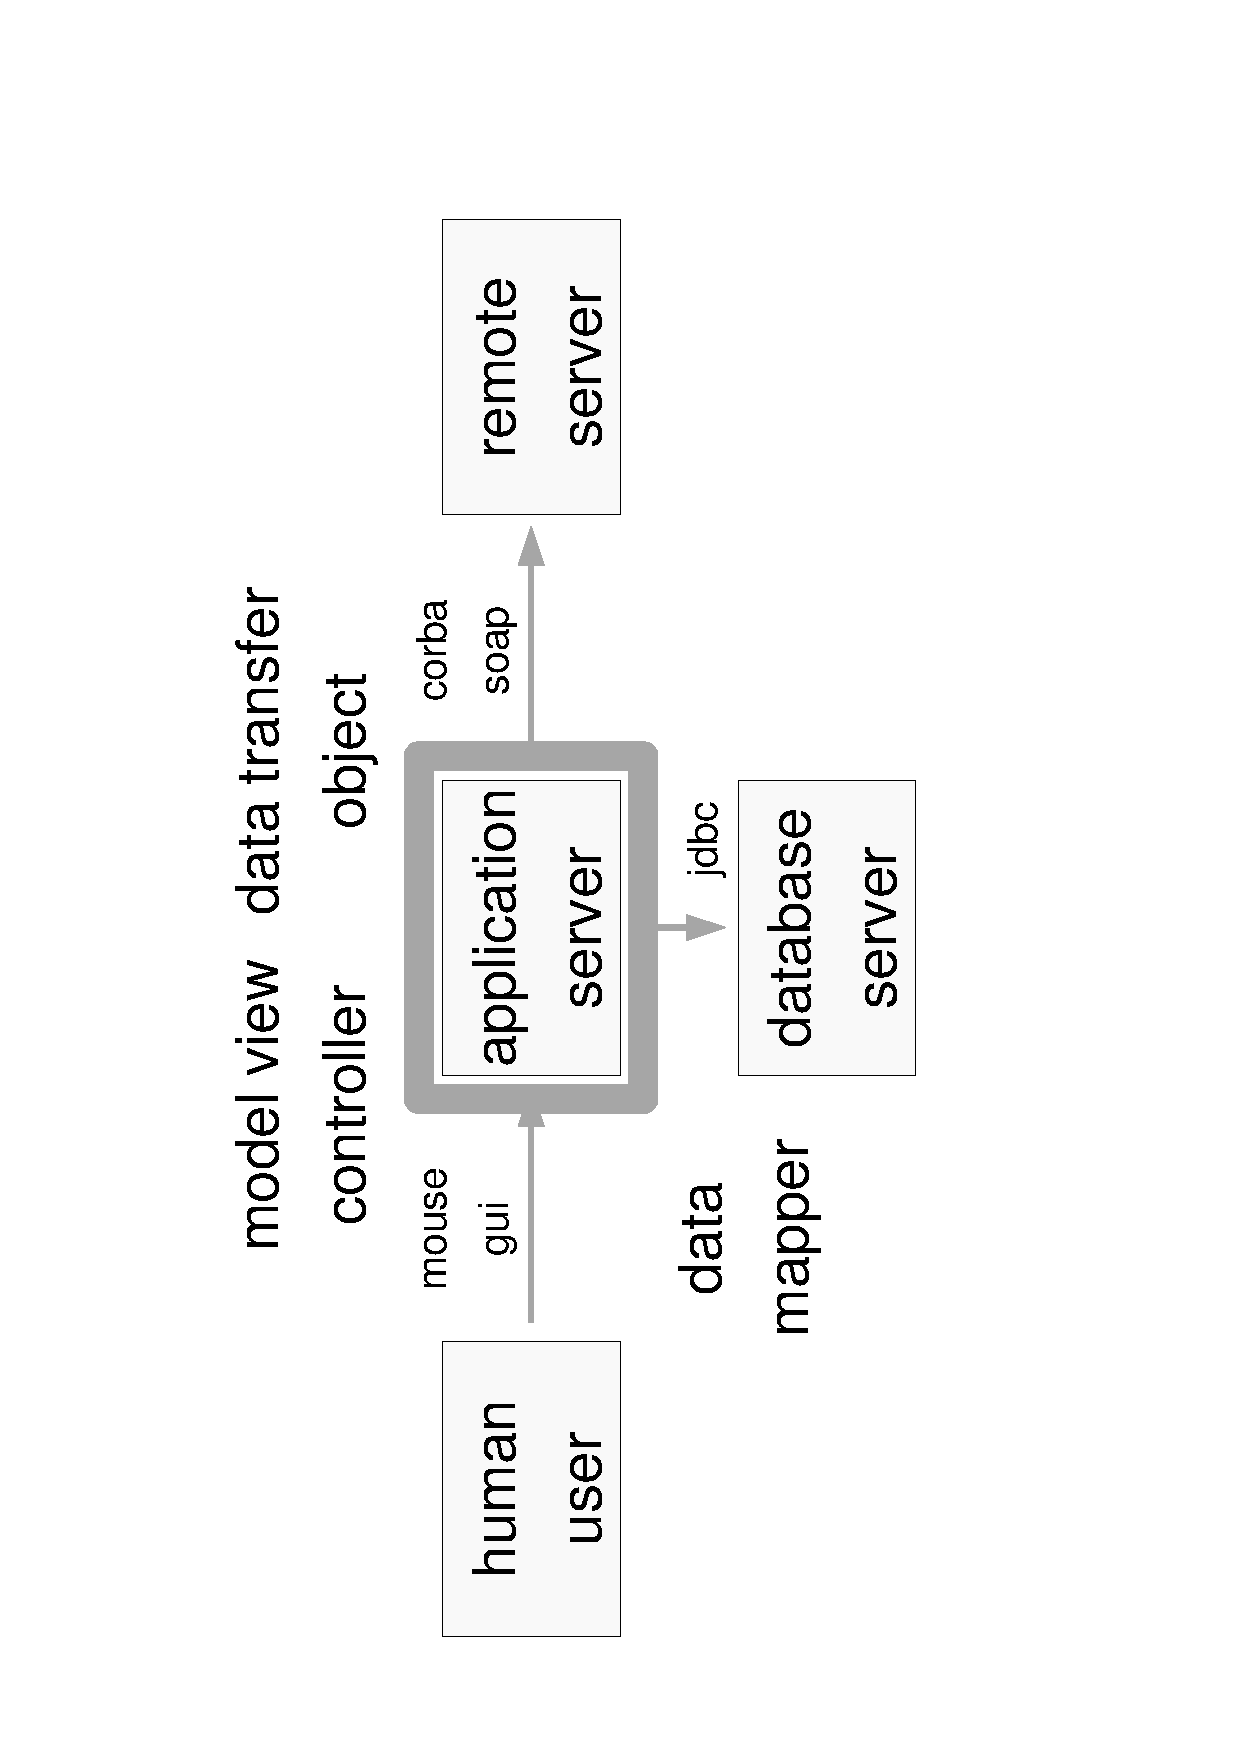
\includegraphics[scale=0.3,angle=-90]{graphic/communication.pdf}
        \caption{IT Environment with Server using Communication Patterns}
        \label{communication_figure}
    \end{center}
\end{figure}

Although software development has become a lot easier in the last decades, it is
still a big effort that should not be underestimated. One thing that application
developers have to care about much of their time is the \emph{Conversion}
between various kinds of (communication) models that a system has:

\begin{itemize}
    \item[-] Frontend (Communication with Human User)
    \item[-] Backend (Communication with Data Source)
    \item[-] Remote (Communication with Server)
    \item[-] Domain (Communication with own Knowledge)
\end{itemize}

The different mechanisms and patterns that have to be considered for such model
conversion often need to be implemented repeatedly, for each new application.
Some trials to unify all backend communication in a common \emph{Persistence Layer}
exist \cite{ambler}, but are remote- and frontend communication seldom considered
in a comparable way. Obviously, no current effort treats the frontend as just
another communication model that has to be \emph{sent} to the human user as
just another system.

The following sections will first reconsider three common communication
patterns, before embedding them into the classical model of logical system
layers (section \ref{layers_heading}). After that, a simplification is
suggested which finally leads to a new \emph{Translator Architecture} (first
introduced in \cite{hellerkunze}).

%
% $RCSfile: basic_patterns.tex,v $
%
% Copyright (c) 2001-2004. Christian Heller. All rights reserved.
%
% No copying, altering, distribution or any other actions concerning this
% document, except after explicit permission by the author!
% At some later point in time, this document is planned to be put under
% the GNU FDL license. For now, _everything_ is _restricted_ by the author.
%
% http://www.cybop.net
% - Cybernetics Oriented Programming -
%
% http://www.resmedicinae.org
% - Information in Medicine -
%
% @author Christian Heller <christian.heller@tuxtax.de>
%

\section{Basic Patterns}
\label{basic_patterns_heading}

%
% $RCSfile: data_mapper.tex,v $
%
% Copyright (c) 2004. Christian Heller. All rights reserved.
%
% No copying, altering, distribution or any other actions concerning this
% document, except after explicit permission by the author!
% At some later point in time, this document is planned to be put under
% the GNU FDL license. For now, _everything_ is _restricted_ by the author.
%
% http://www.cybop.net
% - Cybernetics Oriented Programming -
%
% http://www.resmedicinae.org
% - Information in Medicine -
%
% @author Christian Heller <christian.heller@tuxtax.de>
%

\paragraph{Data Mapper}
\label{data_mapper_heading}

Besides the \emph{Domain Logic}, standard three-tier architectures contain a
\emph{Data Source} layer which may for example represent a database. Both layers
need to exchange data. Modern systems use OOP methods to implement the domain
model. Database models, on the other hand, are often implemented as
\emph{Entity Relationship Model} (ERM).

In order to avoid close coupling and a mix-up of both layers, the introduction
of an additional \emph{Data Mapper} layer \cite{fowler2002} in between the two
others may be justified (figure \ref{datamapper_figure}). The most important
idea of this pattern is to abolish the interdependencies of domain- and
persistence model (database).

\begin{figure}[ht]
    \begin{center}
        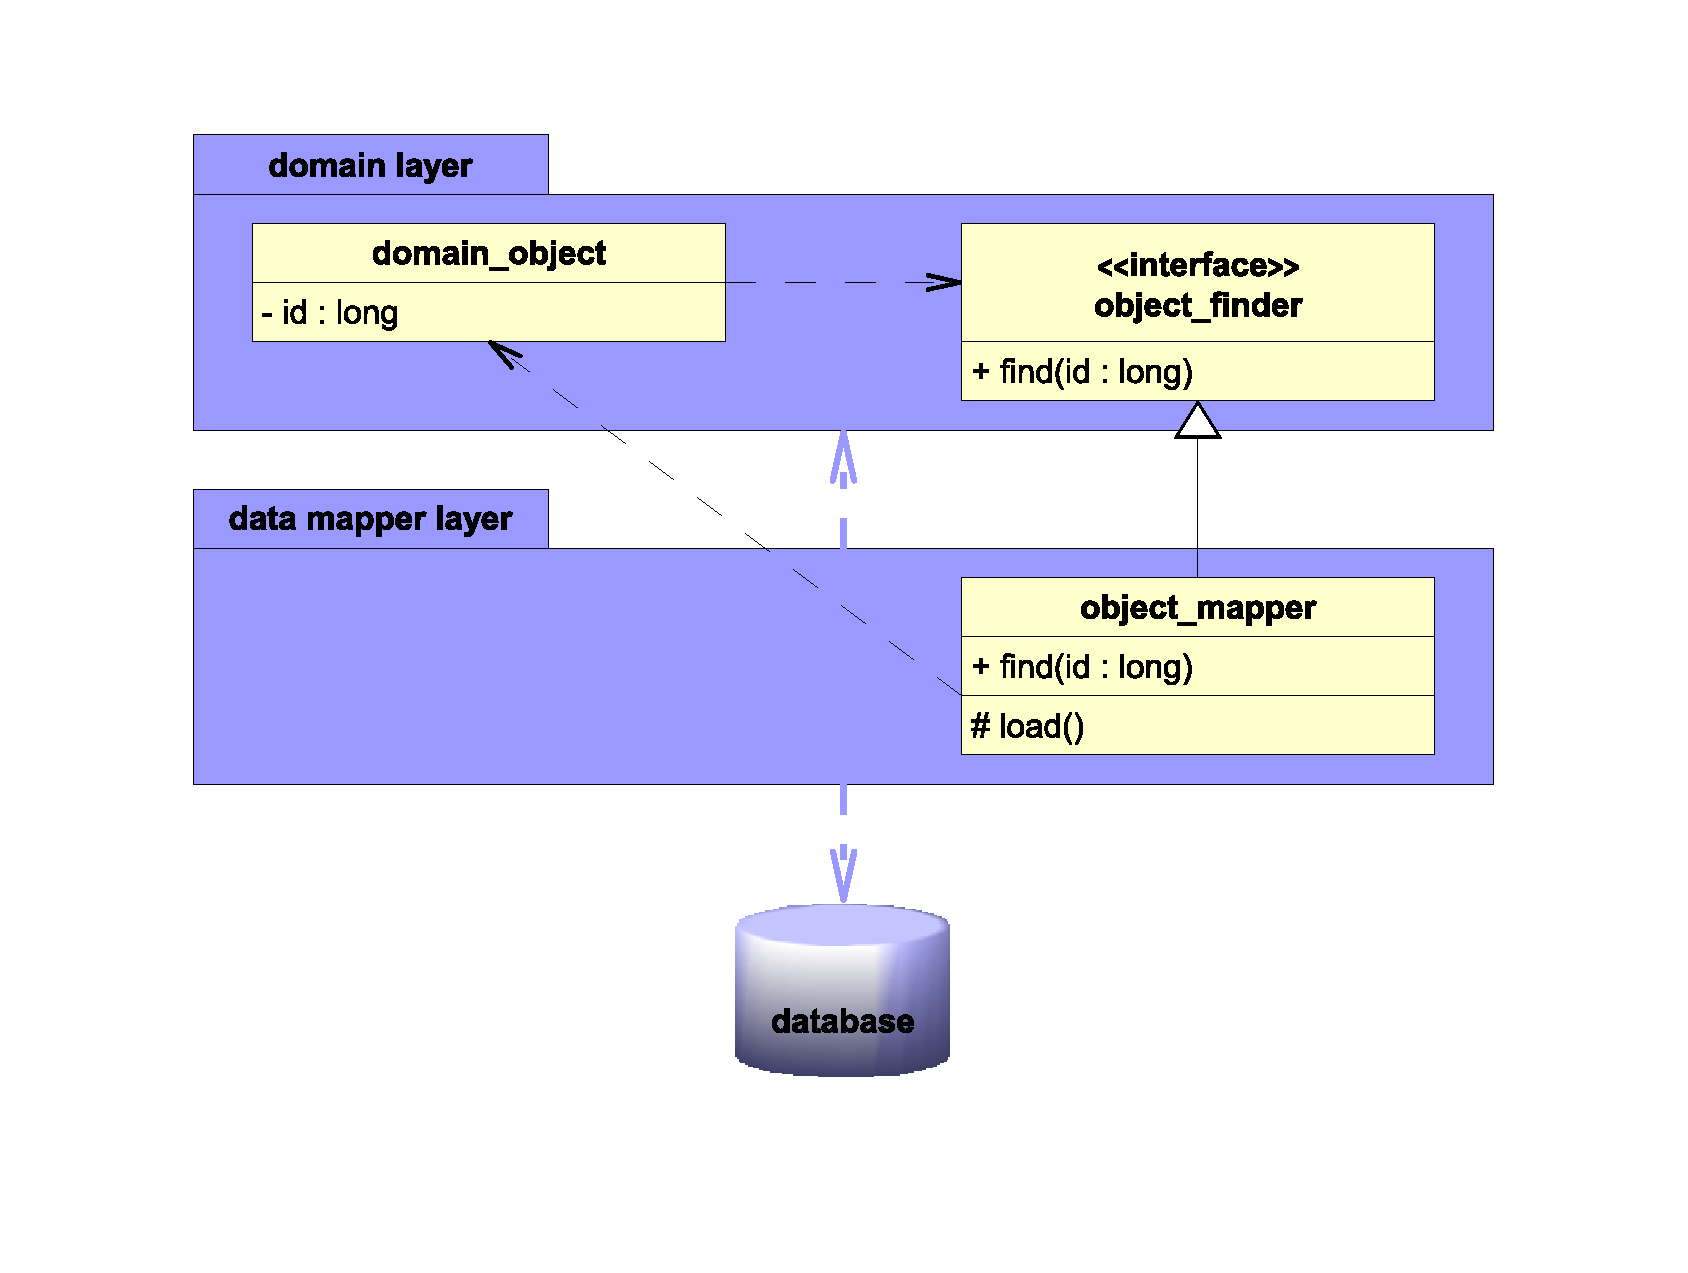
\includegraphics[scale=0.3]{vector/datamapper.eps}
        \caption{Data Mapper Pattern}
        \label{datamapper_figure}
    \end{center}
\end{figure}

The dashed arrows in figure \ref{datamapper_figure} indicate dependencies. The
data mapper layer knows the domain model- as well as the data source layer, via
\emph{unidirectional} relations. Its task is to \emph{translate} between the two,
in both directions. Domain model and data source know nothing from each other.

Each domain model class knows its appropriate interface (\emph{object\_finder})
but does not know the implementation of the same. That is, persistence- and
data retrieval mechanisms are hidden in front of the domain model. The
implementation (\emph{object\_mapper}) is part of the mapping package and also
implements all finder methods. It maps data of the received result sets to the
special attributes of the domain model objects.

The \emph{Mediator} pattern \cite{gamma1995} is similar to the \emph{Mapper}, in
that it is used to decouple different parts of a system. Fowler \cite{fowler2002}
writes: \textit{\ldots the objects that use a mediator are aware of it, even if
they aren't aware of each other; the objects that a mapper separates aren't even
aware of the mapper.}

Although the \emph{Data Mapper} pattern is very helpful at implementing OO
systems, two things are to be criticised:

Firstly, since the \emph{object\_finder} relies on functionality specific to the
retrieval of persistent data, it does actually belong into the data mapper layer
what, if done, would create bidirectional dependencies between the domain model-
and data mapper layer. But also with the \emph{object\_finder} remaining in the
domain model layer, dependencies are not purely unidirectional. It is true that
from an OO view, they are. Internally, however, a super class or interface
relates to its inheriting classes, so that it can call their methods to satisfy
the polymorphic behaviour.

Secondly, the layers do not truely build on each other. Taken a standard
architecture consisting of the following five -- instead of only three -- layers:

\begin{enumerate}
    \item Presentation
    \item Application Process
    \item Domain Model
    \item Data Mapper
    \item Data Source
\end{enumerate}

\ldots the application process does not only access the domain model layer, it
also has to manage (create and destroy) the objects of the data mapper layer.
In other words, it surpasses (disregards) the domain model layer when accessing
the data mapper layer directly.

%
% $RCSfile: data_transfer_object.tex,v $
%
% Copyright (C) 2002-2008. Christian Heller.
%
% Permission is granted to copy, distribute and/or modify this document
% under the terms of the GNU Free Documentation License, Version 1.1 or
% any later version published by the Free Software Foundation; with no
% Invariant Sections, with no Front-Cover Texts and with no Back-Cover
% Texts. A copy of the license is included in the section entitled
% "GNU Free Documentation License".
%
% http://www.cybop.net
% - Cybernetics Oriented Programming -
%
% http://www.resmedicinae.org
% - Information in Medicine -
%
% Version: $Revision: 1.1 $ $Date: 2008-08-19 20:41:06 $ $Author: christian $
% Authors: Christian Heller <christian.heller@tuxtax.de>
%

\subsubsection{Data Transfer Object}
\label{data_transfer_object_heading}
\index{Data Transfer Object Pattern}
\index{DTO}
\index{Assembler Object}
\index{Flat Data Structure}
\index{Translator Architecture}

\begin{figure}[ht]
    \begin{center}
       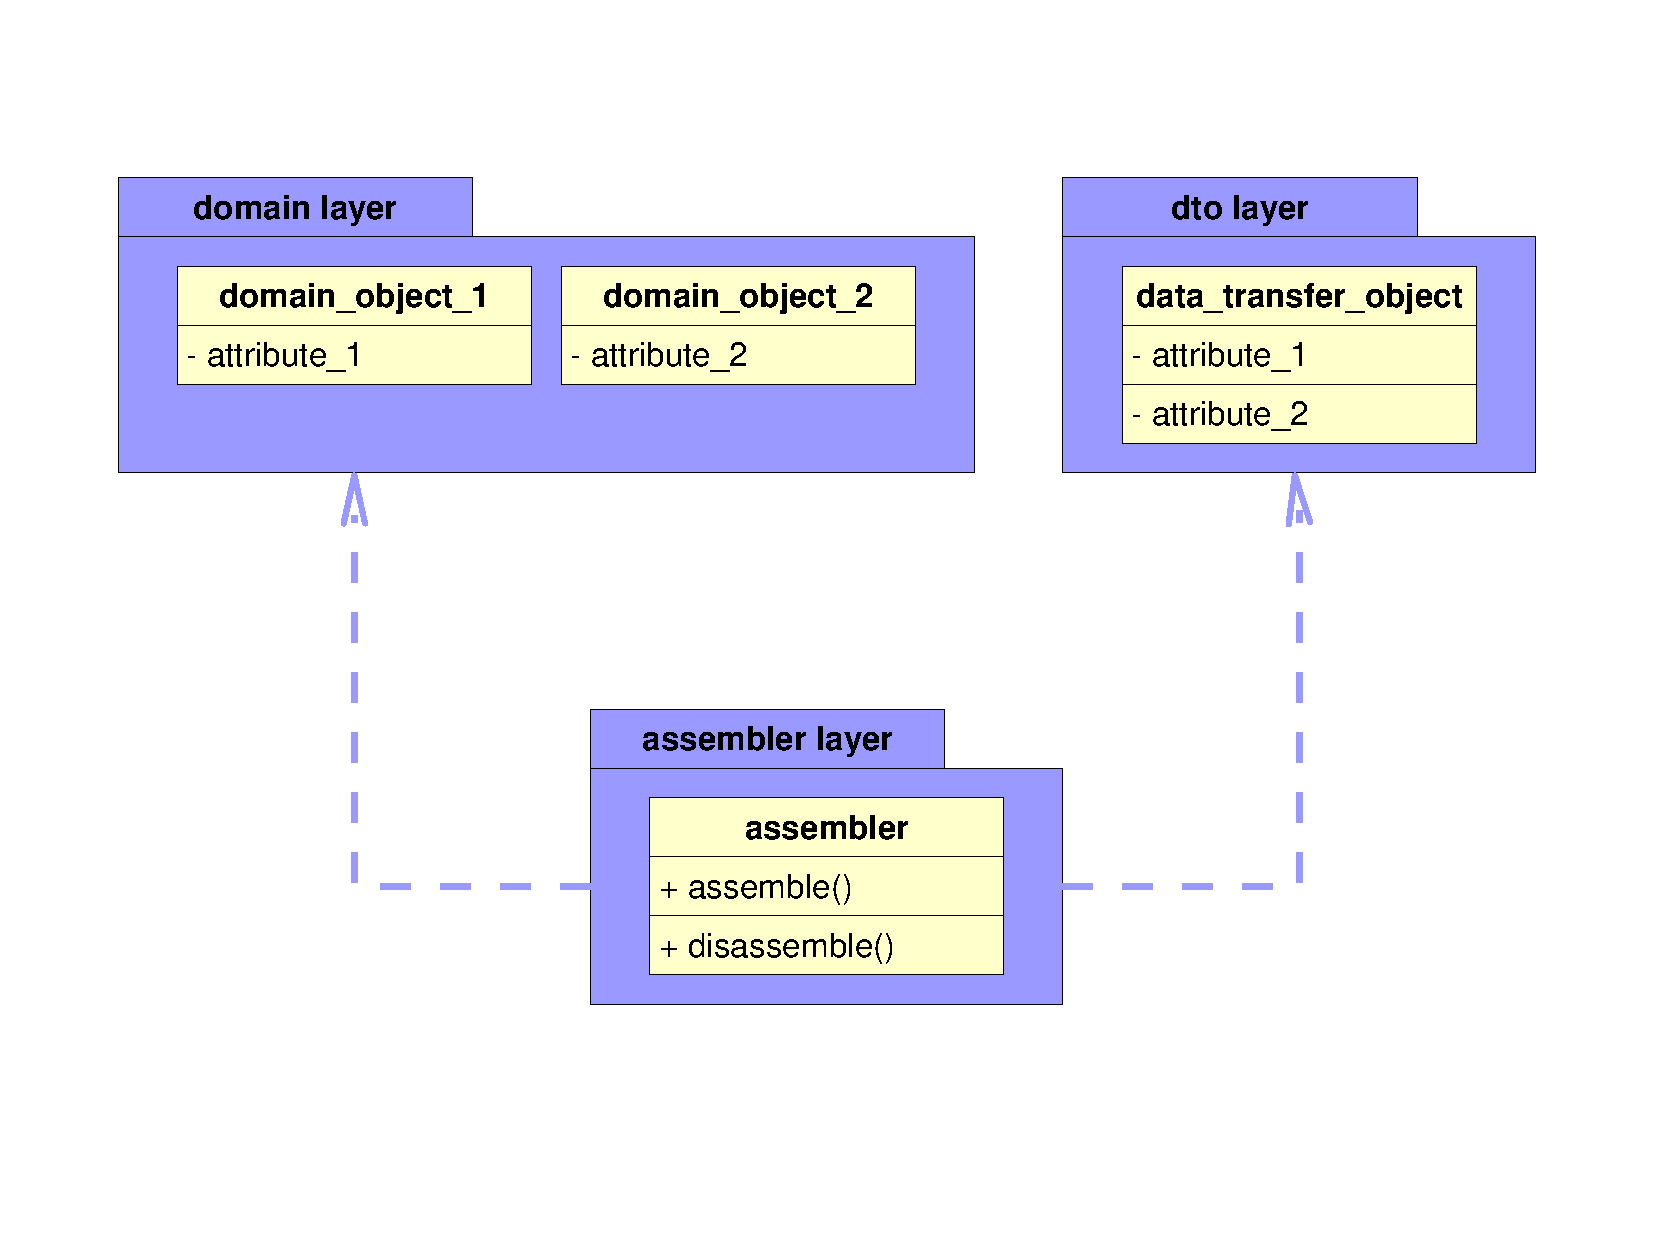
\includegraphics[scale=0.3,angle=-90]{graphic/dto.pdf}
       \caption{Data Transfer Object Pattern}
       \label{dto_figure}
    \end{center}
\end{figure}

It is a well-known fact that many small requests between two processes, and
even more between two hosts in a network need a lot of time. A local machine
with two processes has to permanently change the \emph{Program Context}; a
network has a lot of \emph{Transfers}. For each request, there is a necessity
of at least \emph{two} transfers -- the \emph{Question} of the client and the
\emph{Answer} of the server. Transfer methods are often expected to deliver
common data such as a Person's address, that is surname, first name, street,
zip-code, town and so on. These information is best retrieved by only
\emph{one} transfer call. That way, the client has to wait only once for a
server response and the server does not get too many single tasks. All address
data (in this example) would best be packaged together and sent back to the
client.

A scenario of that kind is exactly what the \emph{Data Transfer Object} pattern
\cite{fowler2002} proposes a solution for: A central \emph{Assembler} object
takes all common data of the server's domain model objects and assembles them
together into a special \emph{Data Transfer Object} (DTO), which is a flat data
structure (figure \ref{dto_figure}). The server will then send this DTO over
network to the client. On the client's side, a similar assembler takes the DTO,
finds out all received data and maps (disassembles) them to the client's domain
model. In that manner, a DTO is able to drastically improve the communication
performance.

Both, \emph{Data Mapper-} and DTO pattern translate one model into another. Due
to this similarity, chapter \ref{state_and_logic_heading} will try to merge
them into a common \emph{Translator} architecture.

%
% $RCSfile: model_view_controller.tex,v $
%
% Copyright (C) 2002-2008. Christian Heller.
%
% Permission is granted to copy, distribute and/or modify this document
% under the terms of the GNU Free Documentation License, Version 1.1 or
% any later version published by the Free Software Foundation; with no
% Invariant Sections, with no Front-Cover Texts and with no Back-Cover
% Texts. A copy of the license is included in the section entitled
% "GNU Free Documentation License".
%
% http://www.cybop.net
% - Cybernetics Oriented Programming -
%
% http://www.resmedicinae.org
% - Information in Medicine -
%
% Version: $Revision: 1.1 $ $Date: 2008-08-19 20:41:07 $ $Author: christian $
% Authors: Christian Heller <christian.heller@tuxtax.de>
%

\subsubsection{Model View Controller}
\label{model_view_controller_heading}
\index{Model View Controller Pattern}
\index{MVC}
\index{Graphical User Interface}
\index{GUI}
\index{Observer Pattern}
\index{Strategy Pattern}
\index{Wrapper Pattern}
\index{Composite Pattern}
\index{Java Foundation Classes}
\index{JFC}
\index{Microsoft Foundation Classes}
\index{MFC}
\index{Document View MVC Variant}
\index{Translator Architecture}

After having had a closer look at design patterns for persistence
(\emph{Data Mapper}) and communication (\emph{Data Transfer Object}), this
section considers the presentation layer of an application (figure
\ref{logical_figure}), which is often realised in form of a
\emph{Graphical User Interface} (GUI). Nowadays, the well-known
\emph{Model View Controller} (MVC) pattern \cite{buschmann, fowler2002} is used
by a majority of standard business applications. Its principle is to have the
\emph{Model} holding domain data, the \emph{View} accessing and displaying
these data and the \emph{Controller} providing the workflow of the application
by handling any action events happening on the view (figure \ref{mvc_figure}).
This separation eases the creation of applications with many synchronous views
on the same data. Internally, the MVC may consist of design patterns like:

\begin{figure}[ht]
    \begin{center}
        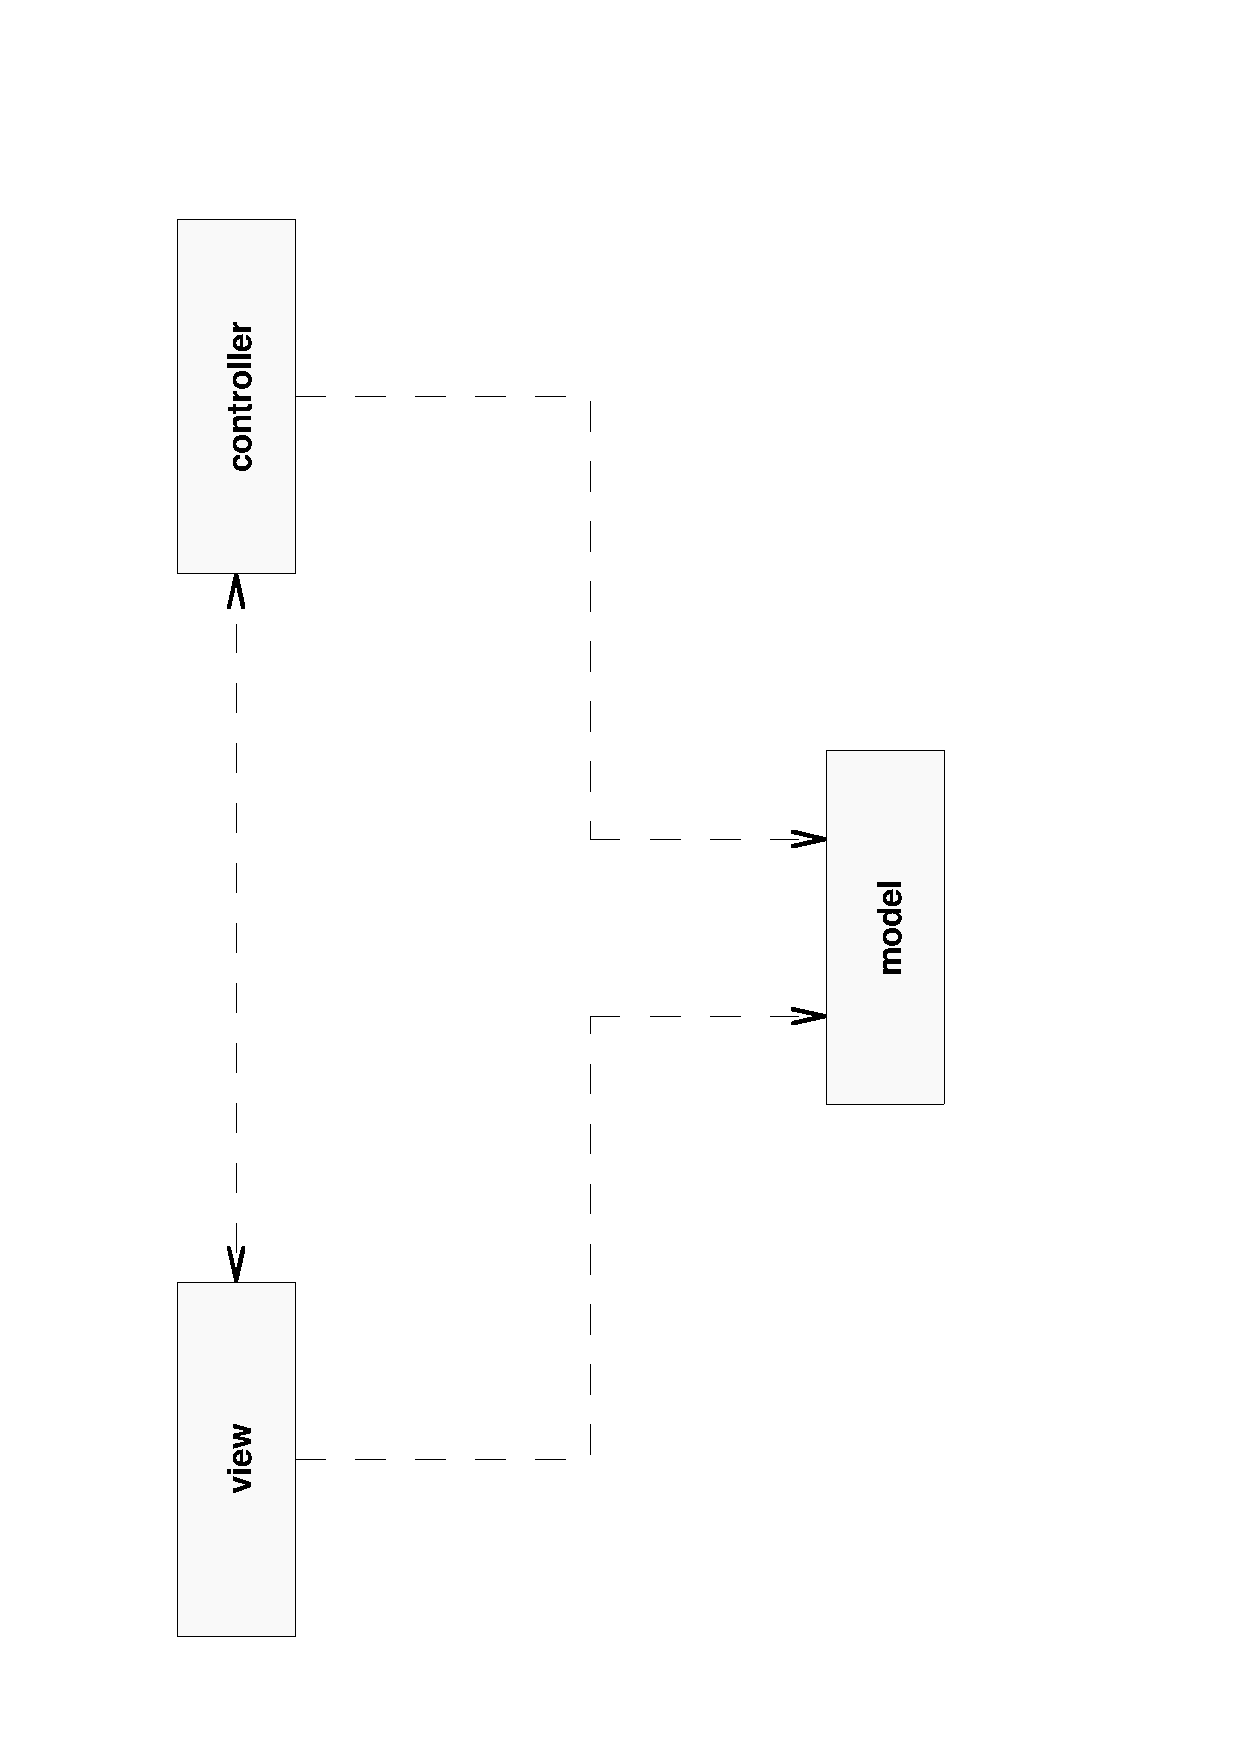
\includegraphics[scale=0.3,angle=-90]{graphic/mvc.pdf}
        \caption{Model View Controller Pattern}
        \label{mvc_figure}
    \end{center}
\end{figure}

\begin{itemize}
    \item[-] \emph{Observer} (section \ref{observer_heading}) which notifies
        the views about data model changes
    \item[-] \emph{Strategy} \cite{gamma1995} which encapsulates exchangeable
        functionality of the controller
    \item[-] \emph{Wrapper} (section \ref{wrapper_heading}) which delegates
        controller functionality to the \emph{Strategy}
    \item[-] \emph{Composite} (section \ref{composite_heading}) which equips
        graphical views with a hierarchical structure
\end{itemize}

Some MVC implementations like parts of the \emph{Java Foundation Classes} (JFC)
use a simplified version not separating controllers from their views. The
\emph{Microsoft Foundation Classes} (MFC) C++ library calls its implementation
\emph{Document-View}.

Besides the above-mentioned patterns \emph{Data Mapper} and DTO, MVC is the
third one getting merged into a common \emph{Translator} architecture, in
chapter \ref{state_and_logic_heading}.



%
% $RCSfile: placement.tex,v $
%
% Copyright (C) 2002-2008. Christian Heller.
%
% Permission is granted to copy, distribute and/or modify this document
% under the terms of the GNU Free Documentation License, Version 1.1 or
% any later version published by the Free Software Foundation; with no
% Invariant Sections, with no Front-Cover Texts and with no Back-Cover
% Texts. A copy of the license is included in the section entitled
% "GNU Free Documentation License".
%
% http://www.cybop.net
% - Cybernetics Oriented Programming -
%
% http://www.resmedicinae.org
% - Information in Medicine -
%
% Version: $Revision: 1.1 $ $Date: 2008-08-19 20:41:08 $ $Author: christian $
% Authors: Christian Heller <christian.heller@tuxtax.de>
%

\subsection{Placement}
\label{placement_heading}
\index{Layered Architecture}
\index{Communication Patterns placed in Layered Architecture}
\index{Model View Controller Pattern}
\index{MVC}
\index{Presentation Layer}
\index{Data Mapper Pattern}
\index{Entity Relationship Model}
\index{ERM}
\index{Database}
\index{DB}
\index{Data Transfer Object}
\index{DTO}
\index{Assembler}

Many state-of-the-art software systems consist of a layered architecture
similar to the one shown in figure \ref{logical_figure}. Yet how do the
communication patterns explained before suit this classical architecture? In
the traditional model of a layered software system, a startable process, best
placed in the \emph{Controller}, creates the whole application tree, to which
belong the \emph{Views} (as user interface), several \emph{Models} of the
\emph{Domain} (providing data to the views and as facade to remote servers) and
the \emph{Data Mapper} (translating between domain- and database model).

\begin{figure}[ht]
    \begin{center}
        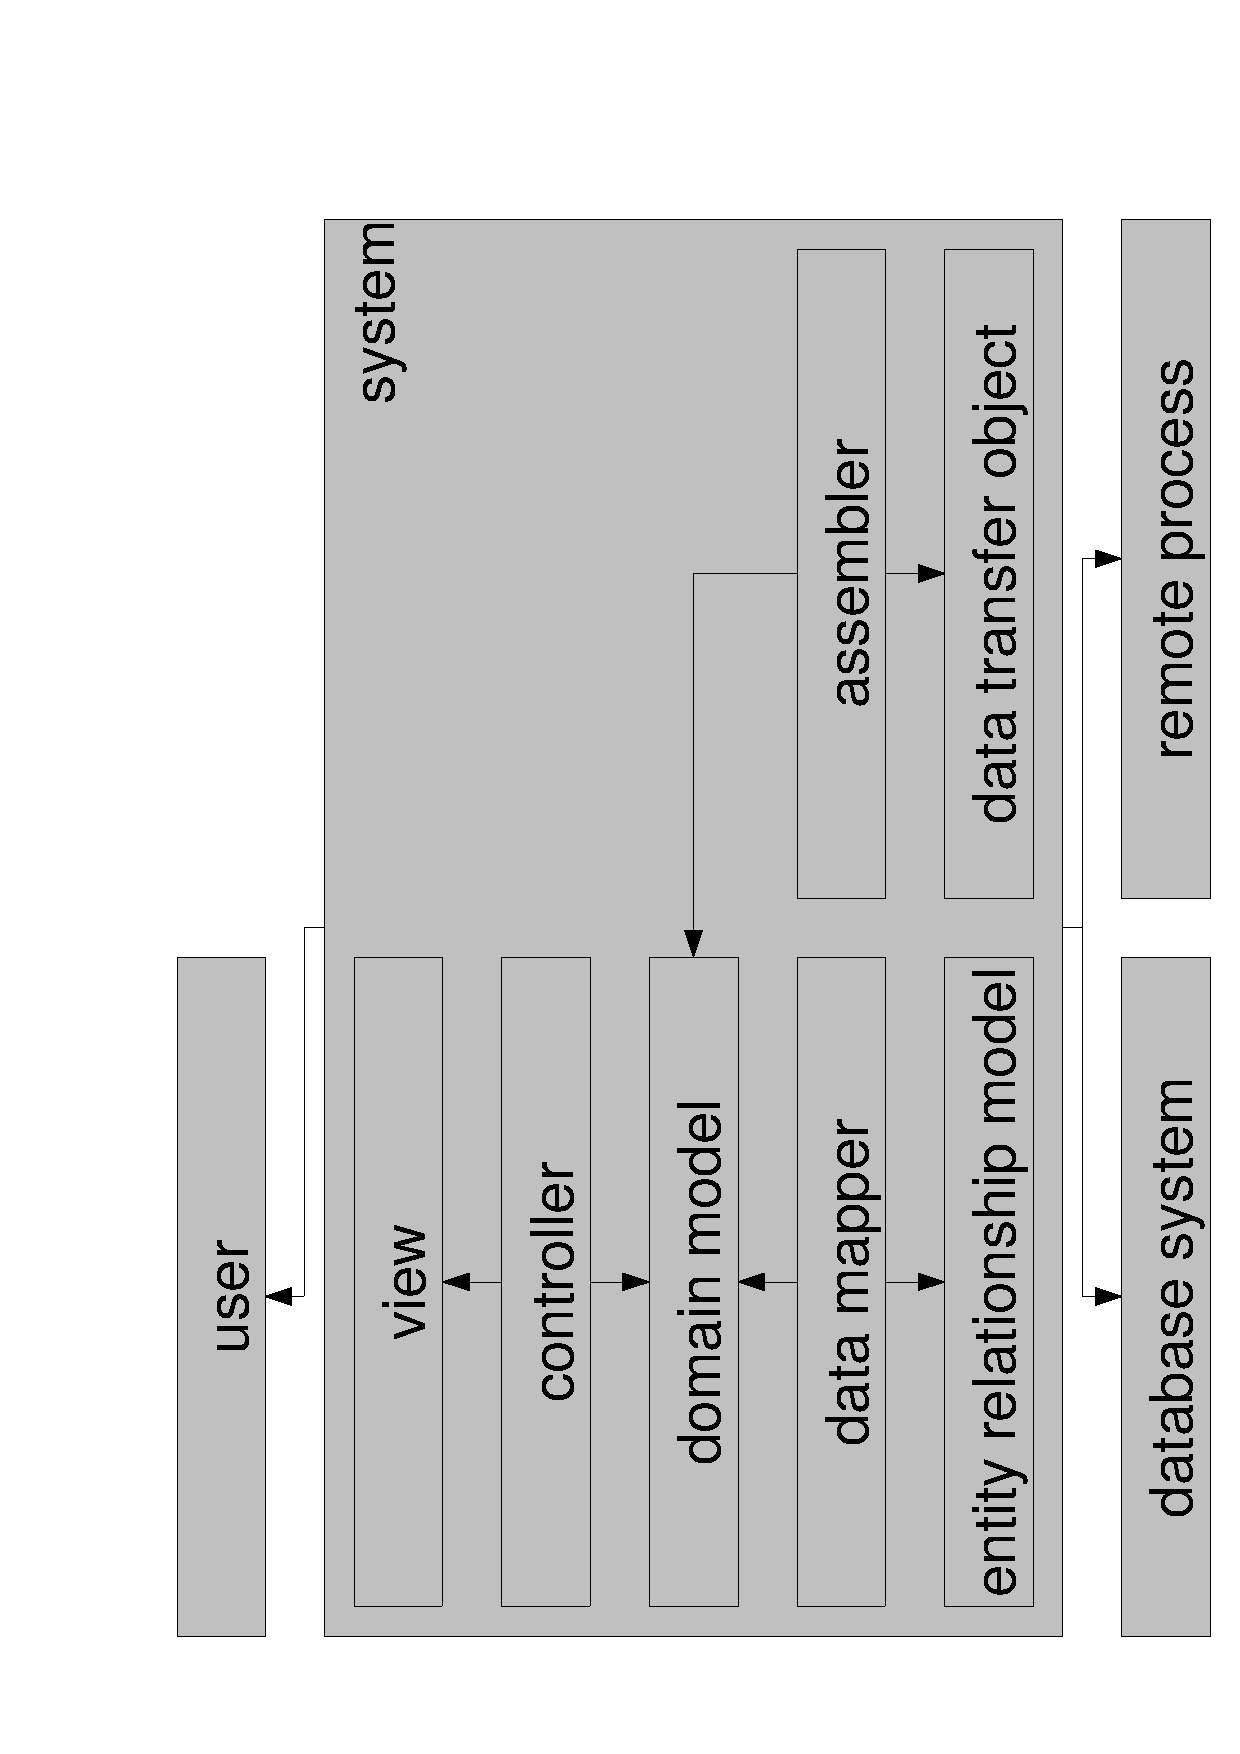
\includegraphics[scale=0.3,angle=-90]{graphic/placement.pdf}
        \caption{Communication Patterns placed in Layered Architecture}
        \label{placement_figure}
    \end{center}
\end{figure}

It is not difficult to figure out where the communication patterns of section
\ref{basic_patterns_heading} fit in here (figure \ref{placement_figure}): The
\emph{Model View Controller} (\emph{Presentation Layer}) determines the parts
to interact with a human user via the \emph{View}; the \emph{Data Mapper}
pattern with its inherent \emph{Entity Relationship Model} (ERM) encapsulates
mechanisms to connect to a persistence medium such as a \emph{Database} (DB);
the \emph{Data Transfer Object} (DTO) and its corresponding assemblers,
finally, serve as means of communication with remote servers.

%
% $RCSfile: simplification.tex,v $
%
% Copyright (C) 2002-2008. Christian Heller.
%
% Permission is granted to copy, distribute and/or modify this document
% under the terms of the GNU Free Documentation License, Version 1.1 or
% any later version published by the Free Software Foundation; with no
% Invariant Sections, with no Front-Cover Texts and with no Back-Cover
% Texts. A copy of the license is included in the section entitled
% "GNU Free Documentation License".
%
% http://www.cybop.net
% - Cybernetics Oriented Programming -
%
% http://www.resmedicinae.org
% - Information in Medicine -
%
% Version: $Revision: 1.1 $ $Date: 2008-08-19 20:41:08 $ $Author: christian $
% Authors: Christian Heller <christian.heller@tuxtax.de>
%

\subsection{Simplification}
\label{simplification_heading}
\index{System as Part of Communication}
\index{Model as Part of Communication}
\index{Translator as Part of Communication}
\index{Simplified Layered Architecture}
\index{State Knowledge}
\index{Logic Knowledge}

For all three kinds of communication, there is a:

\begin{itemize}
    \item[-] \emph{System} (Human User, Database, Remote Server)
    \item[-] \emph{Model} (View, ERM, DTO)
    \item[-] \emph{Translator} (Controller/ View Assembler, Data Mapper, DTO Assembler)
\end{itemize}

\begin{figure}[ht]
    \begin{center}
        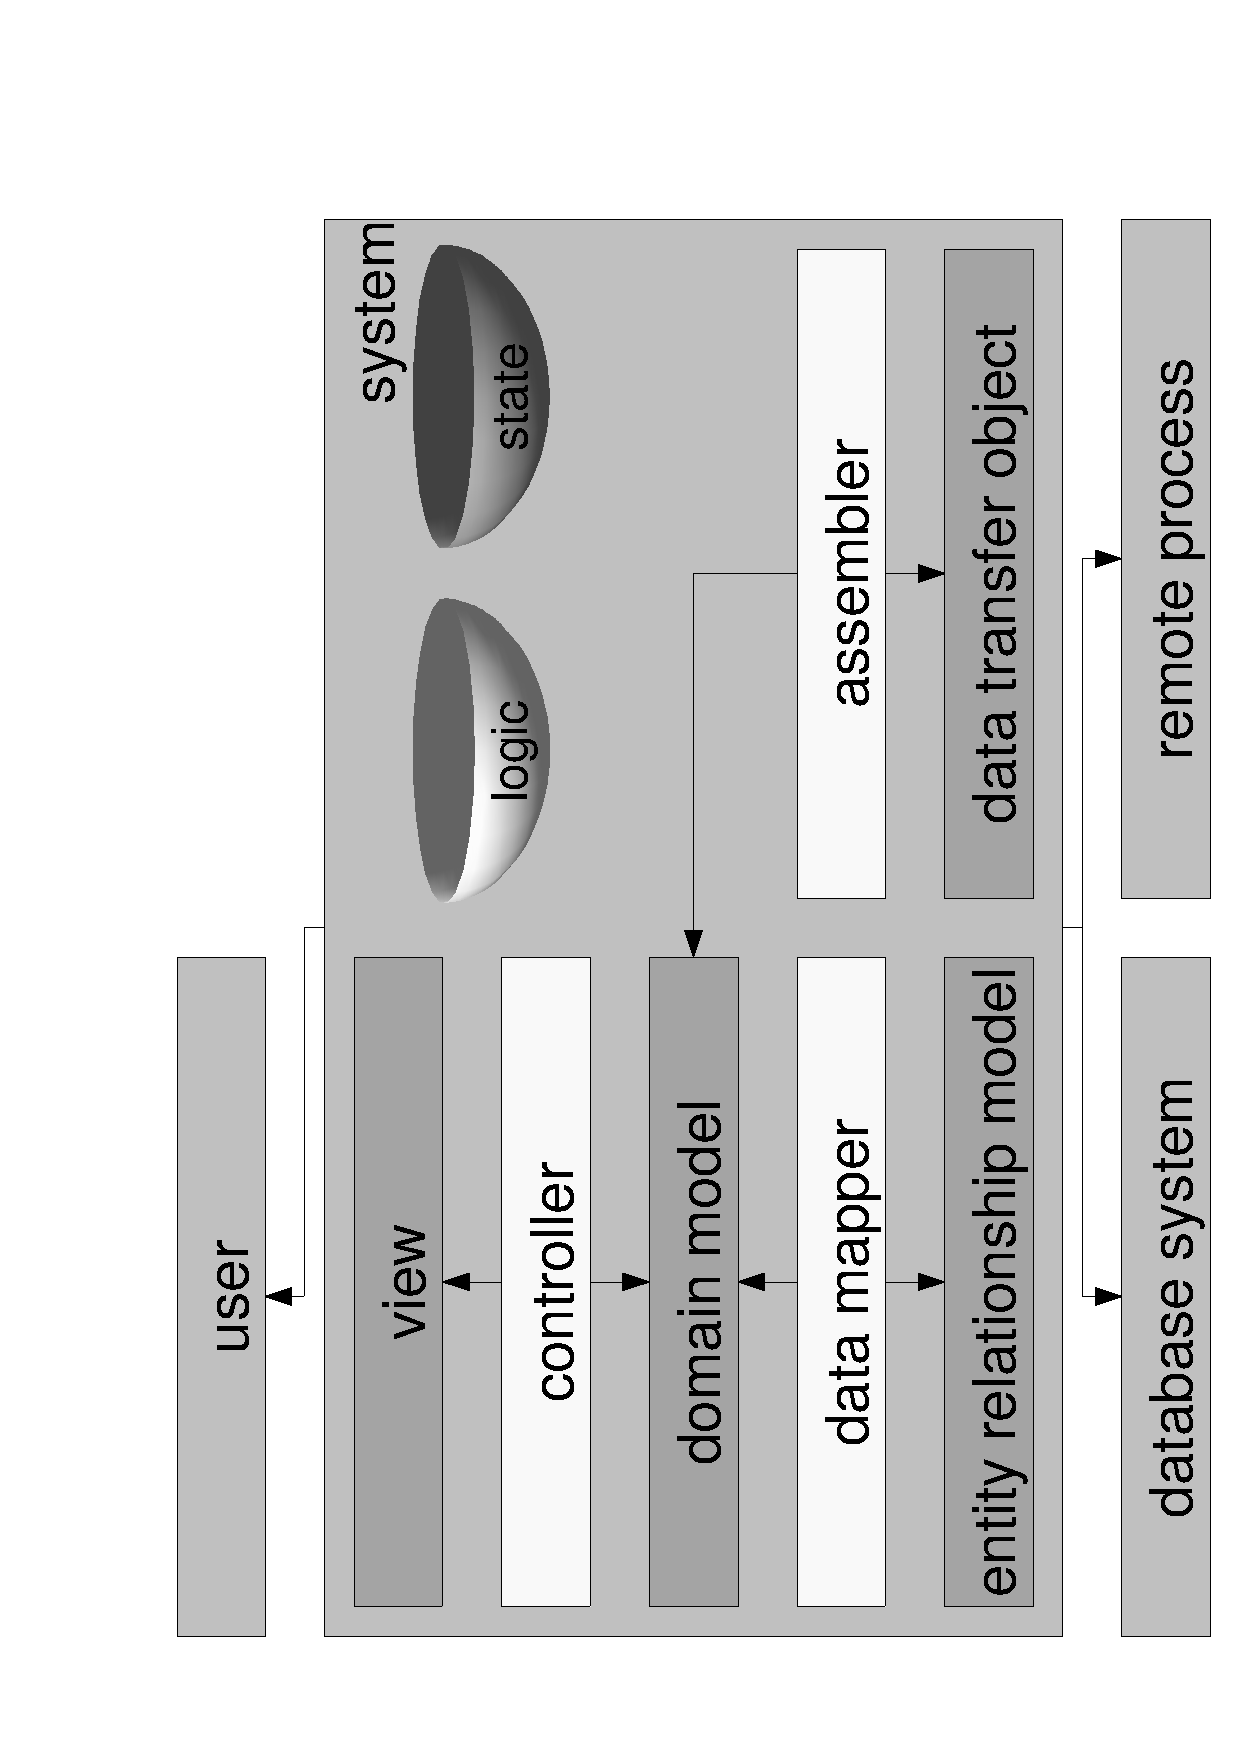
\includegraphics[scale=0.3,angle=-90]{graphic/simplification.pdf}
        \caption{Simplified Layered Architecture with State-/ Logic Knowledge}
        \label{simplification_figure}
    \end{center}
\end{figure}

All models represent certain states; all translators contain logic for
converting one state into another; all systems host their own, specific pool of
state- and logic knowledge. Realising this, a much clearer view on software
architectures can be retrieved (figure \ref{simplification_figure}).

Existing communication patterns can be merged into this common architecture.
Although these patterns suggest their very own communication paradigms, the
basic principles of interaction, as investigated on the example of transient
and persistent communication of humans in section \ref{communication_heading},
remain the same:

\begin{quote}
    An active \emph{System} (concrete process) has a mental state represented
    by passive \emph{Knowledge}. In order to exchange information with another
    system, it translates parts of its domain- into a special communication
    model which it sends to the other system. This is done by accessing its
    hardware infrastructure with \emph{input/ output} (i/o) abilities. The
    other system receives the communication model and translates it back to its
    own domain model.
\end{quote}

Because domain models differ between systems, each system needs its own
translator models. Only communication models need to be agreed upon between
systems; they need to be understood by both communication partners.

%
% $RCSfile: communication_model.tex,v $
%
% Copyright (C) 2002-2008. Christian Heller.
%
% Permission is granted to copy, distribute and/or modify this document
% under the terms of the GNU Free Documentation License, Version 1.1 or
% any later version published by the Free Software Foundation; with no
% Invariant Sections, with no Front-Cover Texts and with no Back-Cover
% Texts. A copy of the license is included in the section entitled
% "GNU Free Documentation License".
%
% http://www.cybop.net
% - Cybernetics Oriented Programming -
%
% http://www.resmedicinae.org
% - Information in Medicine -
%
% Version: $Revision: 1.1 $ $Date: 2008-08-19 20:41:05 $ $Author: christian $
% Authors: Christian Heller <christian.heller@tuxtax.de>
%

\subsection{Communication Model}
\label{communication_model_heading}
\index{Communication Model}
\index{Medium of Communication}
\index{Domain Model}
\index{Transfer Model}
\index{Model Translator}
\index{Mapping Rules}
\index{Notation}
\index{Rules of Translation}
\index{Textual User Interface}
\index{TUI}
\index{Graphical User Interface}
\index{GUI}
\index{Web User Interface}
\index{WUI}
\index{x Datentr\"ager}
\index{xDT}
\index{Healthcare Xchange Protocol}
\index{HXP}
\index{Clinical Document Architecture}
\index{CDA}

As section \ref{communication_heading} pointed out, systems (alive or not)
never communicate directly, but always across the detour of an external
(transient or persistent) \emph{Medium}. This makes it necessary to use special
\emph{Communication Models}, since nearly always, only \emph{parts} of a
complete \emph{Domain Model} want to be exchanged. The use of communication
(transfer) models again, entails the use of model \emph{Translators}. Sowa
\cite{sowa} writes in his book \emph{Knowledge Representation}:

\begin{quote}
    In computer science, there is no end to the number of specialized notations.
    Besides the hundreds of programming languages, there are diagrams for circuits,
    flowcharts, parse trees, game trees, Petri nets, PERT charts, neural networks,
    design languages, and novel notations that are invented whenever two
    programmers work out ideas at the blackboard. Musical notation \ldots\
    is an example of a complex language that is both precise and human factored.
    As long as the mapping rules are defined, all of these notations can be
    automatically translated to or from logic.
\end{quote}

\begin{figure}[ht]
    \begin{center}
        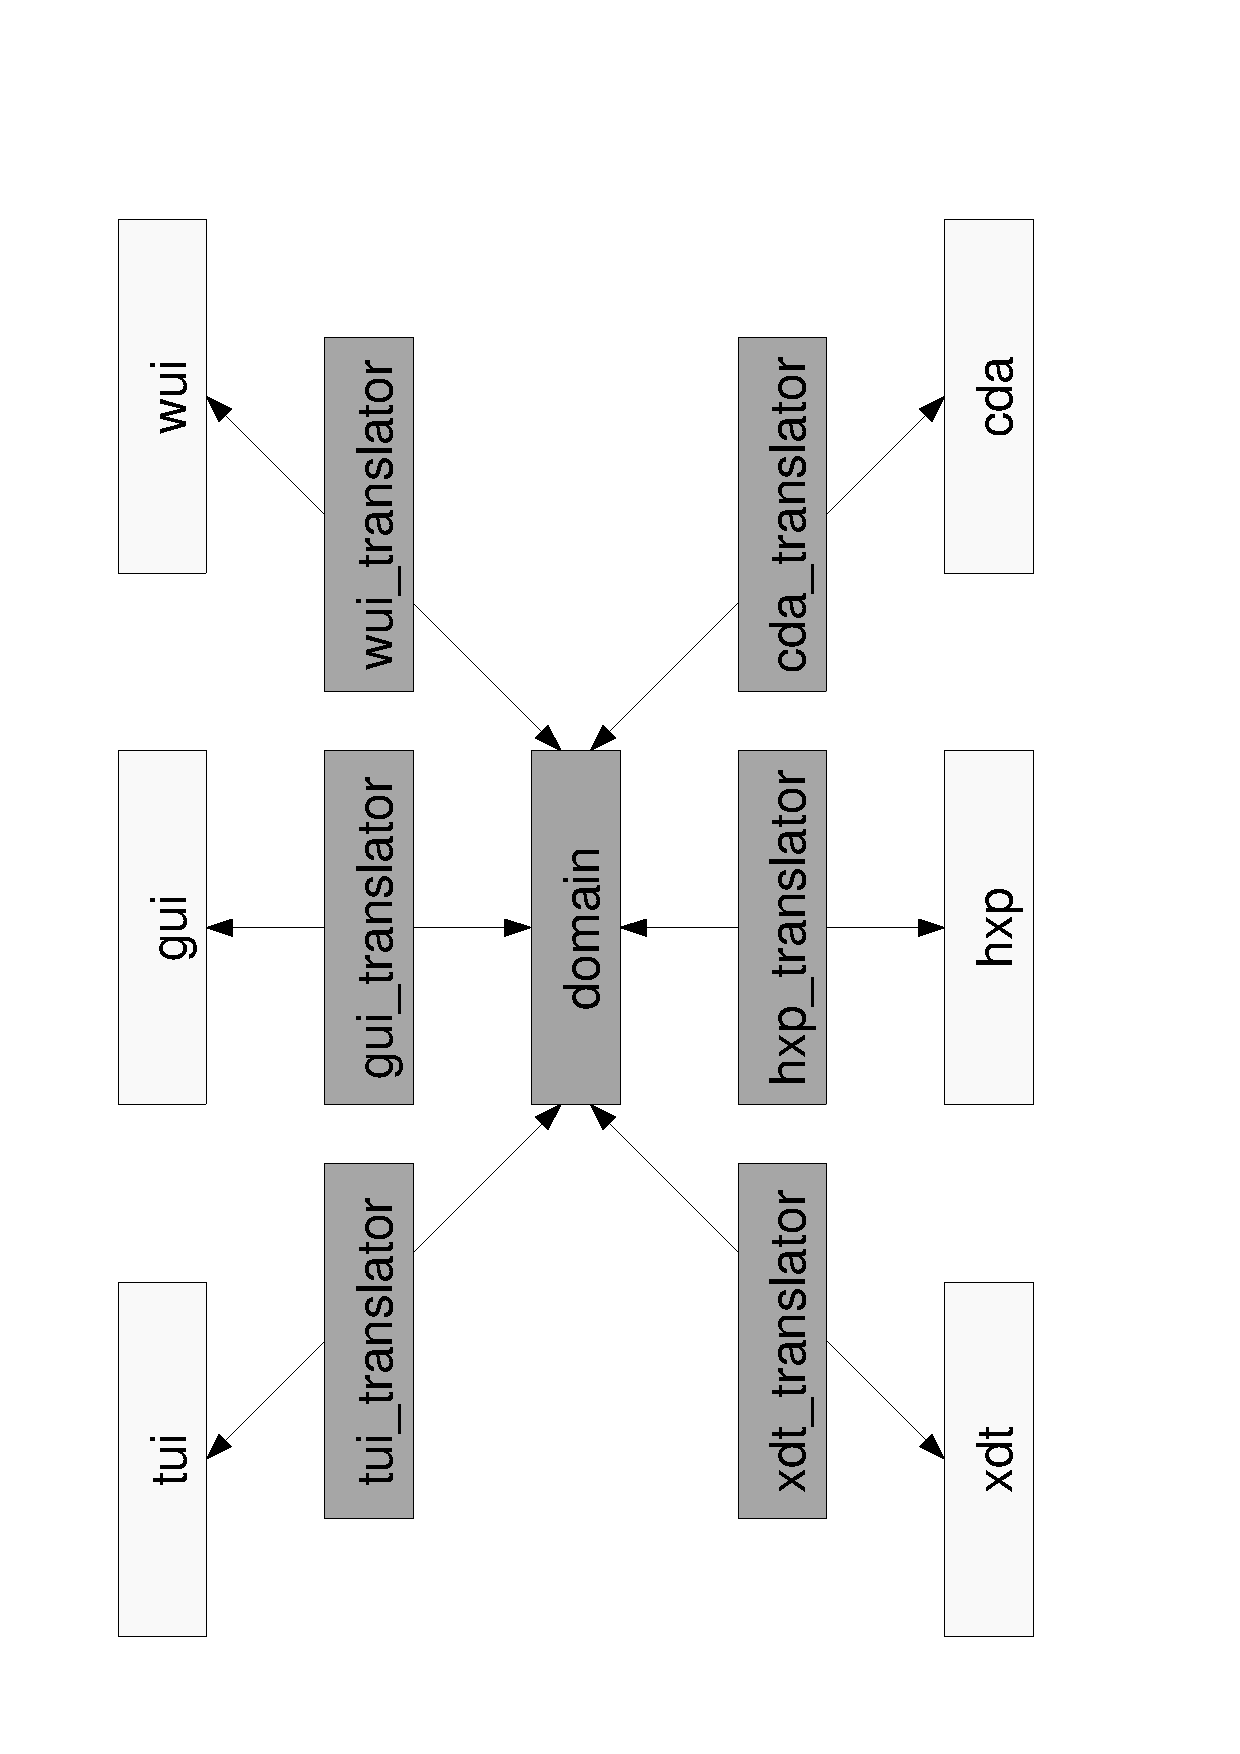
\includegraphics[scale=0.3,angle=-90]{graphic/translators.pdf}
        \caption{Different Kinds of Model Translators}
        \label{translators_figure}
    \end{center}
\end{figure}

Although he does not talk of \emph{Domain-} and \emph{Communication Models},
but of \emph{Notations}, Sowa obviously means the same: Any kind of abstract
model can be translated into any other kind, as long as the translation
\emph{Rules} are defined. Model \emph{Translators} are able to map domain model
data to transfer model data. Depending on which communication style is used,
different translators with different rules need to be applied.

Figure \ref{translators_figure} shows a number of possible model translators,
for a: \emph{Textual User Interface} (TUI), \emph{Graphical User Interface}
(GUI) and \emph{Web User Interface} (WUI) as well as for the German standard
file format for exchanging medical data called \emph{x Datentr\"ager} (xDT),
the \emph{Healthcare Xchange Protocol} (HXP) and HL7's exchange format called
\emph{Clinical Document Architecture} (CDA). More on these standards in chapter
\ref{res_medicinae_heading}.

Many application systems have exactly one domain model but transfer models of
arbitrary type should be addable anytime. Translators only know how to
translate between the domain model and a special transfer model, of course in
both directions. \emph{Direct} translation between transfer models is an
exception; it is possible but better done \emph{via} the domain model.

The type of transfer model is independent from the communication mechanism
used. The usage of a \emph{Graphical User Interface} (GUI) model, for example,
is not necessarily limited to human-computer interaction. It could very well be
used for data transfer between remote computers, as long as both systems know
how to translate that model.

%%
% $RCSfile: knowledge_split.tex,v $
%
% Copyright (C) 2002-2008. Christian Heller.
%
% Permission is granted to copy, distribute and/or modify this document
% under the terms of the GNU Free Documentation License, Version 1.1 or
% any later version published by the Free Software Foundation; with no
% Invariant Sections, with no Front-Cover Texts and with no Back-Cover
% Texts. A copy of the license is included in the section entitled
% "GNU Free Documentation License".
%
% http://www.cybop.net
% - Cybernetics Oriented Programming -
%
% http://www.resmedicinae.org
% - Information in Medicine -
%
% Version: $Revision: 1.1 $ $Date: 2008-08-19 20:41:07 $ $Author: christian $
% Authors: Christian Heller <christian.heller@tuxtax.de>
%

\subsection{Knowledge Split}
\label{knowledge_split_heading}

refer back to section \ref{input_output_and_rules_heading}

The \emph{Knowledge Query and Manipulation Language} (KQML) (section
\ref{knowledge_query_and_manipulation_language_heading}), a popular means of
communication in \emph{Agent Oriented Programming} (section
\ref{agent_oriented_programming_heading}), relies on \emph{Speech Act Theory}
developed by Searle 1960 and enhanced by Winograd and Flores in the 70s.
\cite{wikipedia} http://en.wikipedia.org/wiki/Agent\_communication\_language

- describe some language differences: CYBOL in comparison to Agent0:
http://www.cs.caltech.edu/~bond/courses/cs101c/agents16/node13.html
(states=believes, logic=capabilities, signal=commitment)
Do Agent0 and others provide the most suitable format to represent knowledge?

Two Comparison Tables:

1 with Agent0

http://www.cs.caltech.edu/~bond/courses/cs101c/agents16/node3.html

Mental State
    Beliefs (= Facts)
        ?? State Knowledge
    Commitments (to act, are grounded, that is do not contain variables)
        pre-defined actions are: DO, INFORM, REQUEST, UNREQUEST, REFRAIN, IF
        ?? Signal (signal removal is called "Release of a Commitment")
    Capabilities (= Actions; Commitments to oneself are special capabilities called Decision or Choice)
        ?? Logic Knowledge

Goals?
Intentions?
Time is treated as realtime; it is expressed explicitly, that is by adding it
to statements.
Action is represented by the fact that it happened at a given time;
since actions are facts they are also instantaneous.
Messages are passed by agents to each other, by message name.

2 with Kuehnel

- can all the different vocabulary (see Kuehnel: action, plan, assumption, aim/goal)
be simplified/unified into an easier system?
- Agents know about the environment and their own expertise
- add table for comparison between CYBOP and AGOP, for example:
    state knowledge = beliefs: capabilities (knowledge about itself)
        + constraints (knowledge about environment)
    logic knowledge = actions + plans
    signal = goal (aim)
- this is a comparison \emph{Trial} -- terms of AGOP are anyway not used uniformly in science

- ideas to split knowledge itself into state- and logic (action/ plan) knowledge
- see \cite[p. 95 ff., p. 125 ff.]{kuehnel}

%%
% $RCSfile: bundling.tex,v $
%
% Copyright (C) 2002-2008. Christian Heller.
%
% Permission is granted to copy, distribute and/or modify this document
% under the terms of the GNU Free Documentation License, Version 1.1 or
% any later version published by the Free Software Foundation; with no
% Invariant Sections, with no Front-Cover Texts and with no Back-Cover
% Texts. A copy of the license is included in the section entitled
% "GNU Free Documentation License".
%
% http://www.cybop.net
% - Cybernetics Oriented Programming -
%
% http://www.resmedicinae.org
% - Information in Medicine -
%
% Version: $Revision: 1.1 $ $Date: 2008-08-19 20:41:05 $ $Author: christian $
% Authors: Christian Heller <christian.heller@tuxtax.de>
%

\subsection{Bundling}
\label{bundling_heading}

OOP
\emph{Classes} as known from \emph{Object Oriented Programming} (OOP) bundle
attributes and methods which often causes additional inter-dependencies in a
system because classes do not only have to relate to other classes for accessing
their attributes but also for using the methods offered by them.

Bean/ Enterprise Java Bean (EJB)

- JMS Eigenschaften werden in EJBs eingebaut, so dass diese selbststaendig
andere EJBs aufrufen koennen.
- Verlagerung eines Teils der Application Logic into domain
--> bliebe nur noch 1 Schicht uebrig, die Domain (Gehirn)
--> Unguenstig, da mehrere verschiedene Sichten auf Domain gewuenscht und notwendig;
daher immer nur Domain-Extracts in Application dargestellt!
- How about adding a GUI to every EJB so that it can be displayed automatically?
--> useless: users want different guis and EJB data need to be displayed in
different contexts
==> the concept of merging more and more functionality into components a la EJB
is not arbitrarily continuable, nor always desired (different views on domain)


%
% $RCSfile: knowledge_abstraction_and_manipulation.tex,v $
%
% Copyright (C) 2002-2008. Christian Heller.
%
% Permission is granted to copy, distribute and/or modify this document
% under the terms of the GNU Free Documentation License, Version 1.1 or
% any later version published by the Free Software Foundation; with no
% Invariant Sections, with no Front-Cover Texts and with no Back-Cover
% Texts. A copy of the license is included in the section entitled
% "GNU Free Documentation License".
%
% http://www.cybop.net
% - Cybernetics Oriented Programming -
%
% http://www.resmedicinae.org
% - Information in Medicine -
%
% Version: $Revision: 1.1 $ $Date: 2008-08-19 20:41:07 $ $Author: christian $
% Authors: Christian Heller <christian.heller@tuxtax.de>
%

\section{Knowledge Abstraction and -Manipulation}
\label{knowledge_abstraction_and_manipulation_heading}
\index{Knowledge Abstraction}
\index{Knowledge Manipulation}

Having shown the existence of state- and logic knowledge, not only in software
systems, and having compared both with a classical layered software architecture,
what is still missing is an overview of fundamental abstractions of state- as
well as logic knowledge, and a solution showing how both can be manipulated, in
a knowledge-based system.

%
% $RCSfile: algorithm.tex,v $
%
% Copyright (C) 2002-2008. Christian Heller.
%
% Permission is granted to copy, distribute and/or modify this document
% under the terms of the GNU Free Documentation License, Version 1.1 or
% any later version published by the Free Software Foundation; with no
% Invariant Sections, with no Front-Cover Texts and with no Back-Cover
% Texts. A copy of the license is included in the section entitled
% "GNU Free Documentation License".
%
% http://www.cybop.net
% - Cybernetics Oriented Programming -
%
% http://www.resmedicinae.org
% - Information in Medicine -
%
% Version: $Revision: 1.1 $ $Date: 2008-08-19 20:41:05 $ $Author: christian $
% Authors: Christian Heller <christian.heller@tuxtax.de>
%

\subsection{Algorithm}
\label{algorithm_heading}
\index{Algorithm}
\index{Knowledge Engineering}
\index{KE}
\index{Ontology}
\index{Knowledge Schema}
\index{State Model}
\index{Logic Model}
\index{Sequence of (Mapping) Rules}
\index{Lambda Calculus}
\index{Turing Machine}

For John F. Sowa \cite{sowa}, \emph{Knowledge Engineering} (KE) is:
\textit{the application of logic and ontology to the task of building
computable models of some domain for some purpose.} Section
\ref{knowledge_representation_heading} showed how an \emph{Ontology} can be
applied to structure state knowledge of a domain, and introduced a new
\emph{Knowledge Schema}. This section investigates the universality of that
knowledge schema, that is its applicability to \emph{State-} as well as
\emph{Logic} models.

Not only input/ output (i/o) knowledge (states) can be structured
hierarchically, using an ontology, the operations of a system (logic) can be
cascaded and nested as well. The resulting logic models are \emph{Sequences} of
input-to-output mapping rules that can consist of yet finer-grained models. The
theory of computing uses the word \emph{Algorithm} to label a sequence of
mapping rules. Banerjee \cite{banerjee} writes on this:

\begin{quote}
    Each \ldots\ mathematician had to precisely define the notion of an
    algorithm, and each defined it in a different way. Godel defined algorithm
    as a \emph{Sequence of Rules} for forming complicated mathematical
    functions out of simple mathematical functions, Church used a formalism
    called the \emph{Lambda Calculus}, while Turing used a mathematical object
    called the \emph{Turing Machine} and defined an algorithm to be any set of
    instructions for his simple machine. All these seemingly different and
    independently contrived definitions turned out to be equivalent and they
    form the basics of the modern theory of computing. No modern programming
    language can achieve more, in principle, than the Turing machine or the
    lambda-calculus.
\end{quote}

\emph{Time} plays an important role in data processing. It dictates the order
in which steps of an algorithm are executed and thereby ensures a correct
sequence of actions. Every element of an algorithm needs to be assigned an
instant (position) in time, as meta information. Although the runtime-processing
of data, according to an algorithm, is \emph{dynamic}, the models of logic --
just like i/o state models -- are \emph{static} (chapter
\ref{statics_and_dynamics_heading}).

%
% $RCSfile: operations.tex,v $
%
% Copyright (C) 2002-2008. Christian Heller.
%
% Permission is granted to copy, distribute and/or modify this document
% under the terms of the GNU Free Documentation License, Version 1.1 or
% any later version published by the Free Software Foundation; with no
% Invariant Sections, with no Front-Cover Texts and with no Back-Cover
% Texts. A copy of the license is included in the section entitled
% "GNU Free Documentation License".
%
% http://www.cybop.net
% - Cybernetics Oriented Programming -
%
% http://www.resmedicinae.org
% - Information in Medicine -
%
% Version: $Revision: 1.1 $ $Date: 2008-08-19 20:41:08 $ $Author: christian $
% Authors: Christian Heller <christian.heller@tuxtax.de>
%

\subsection{Operations}
\label{operations_heading}
\index{Operation}
\index{Binary Arithmetic}
\index{Digital Logic Circuit}
\index{Two's Complement}
\index{AND Operation}
\index{Boolean Operation}
\index{Comparison Operation}
\index{Arithmetic Operation}

In the end, all computer-implemented procedures go back to boolean operations
and binary arithmetic (section \ref{from_philosophy_to_mathematics_heading}),
processed by digital logic circuits (section \ref{digital_logic_heading}). A
\emph{Multiplication} can be expressed as sequence of additions. By
representing the number to be subtracted in its negative form
(\emph{Two's Complement} \cite{philippow}), a \emph{Subtraction} can be mapped
to an addition. An \emph{Addition} itself is performed by linking Bits of the
summands logically, using an \emph{AND} operation. Fundamental operations for
knowledge translation are:

\begin{itemize}
    \item[-] \emph{Boolean:} and, or
    \item[-] \emph{Comparison:} equal, smaller, greater
    \item[-] \emph{Arithmetic:} add, subtract, multiply, divide
\end{itemize}

They all imply special rules after which one or more input operands (values)
get transformed into one or more output operands. Both kinds representing
static \emph{State Models}, input and output can be placed as branches of one
common knowledge tree. But also the rules as static \emph{Logic Models} can be
added to this tree.

%
% $RCSfile: primitives.tex,v $
%
% Copyright (C) 2002-2008. Christian Heller.
%
% Permission is granted to copy, distribute and/or modify this document
% under the terms of the GNU Free Documentation License, Version 1.1 or
% any later version published by the Free Software Foundation; with no
% Invariant Sections, with no Front-Cover Texts and with no Back-Cover
% Texts. A copy of the license is included in the section entitled
% "GNU Free Documentation License".
%
% http://www.cybop.net
% - Cybernetics Oriented Programming -
%
% http://www.resmedicinae.org
% - Information in Medicine -
%
% Version: $Revision: 1.1 $ $Date: 2008-08-19 20:41:08 $ $Author: christian $
% Authors: Christian Heller <christian.heller@tuxtax.de>
%

\subsection{Primitives}
\label{primitives_heading}
\index{Primitive}
\index{State Primitive}
\index{Binary Digit}
\index{Bit}
\index{Byte}
\index{Word}
\index{Double Word}
\index{File}
\index{Hard Disk Drive}
\index{HDD}
\index{Random Access Memory}
\index{RAM}
\index{Multipurpose Internet Mail Extension}
\index{MIME}
\index{Text MIME Type}
\index{Image MIME Type}
\index{Audio MIME Type}
\index{Video MIME Type}
\index{Application MIME Type}

All software is based on the final two states called \emph{one} \& \emph{zero},
or \emph{on} \& \emph{off}, or \emph{true} \& \emph{false}, or similarly. A
\emph{Binary Digit} (Bit) can take on the values \emph{zero} or \emph{one}; it
represents the final abstraction of any software model and can be easily mapped
to hardware. A second unit, the \emph{Byte}, consists of eight Bits. One
\emph{Word} is made up of two Bytes, one \emph{Double Word} of four Bytes and
so forth. Data in a \emph{File} on a \emph{Harddisk Drive} (HDD) partition or
another storage medium are saved in form of Bit sequences, just like data in
\emph{Random Access Memory} (RAM). It is up to a program to interpret these
data correctly, in the desired manner.

\begin{figure}[ht]
    \begin{center}
        \begin{footnotesize}
        \begin{tabular}{| p{70mm} | p{35mm} |}
            \hline
            \textbf{Primitivum} & \textbf{Size} [Byte]\\
            \hline
            Date, Time, Complex, Fraction, Term & many\\
            \hline
            Double, Float, Vector, String & 8, 12, 16 or more\\
            \hline
            Integer, Pointer, Word, Short, Byte, Character & 1, 2, 4, 7, 8 or more\\
            \hline
            Bit, Boolean & 0 or 1 Bit\\
            \hline
        \end{tabular}
        \end{footnotesize}
        \caption{State Primitives sorted after their Granularity}
        \label{primitives_table}
    \end{center}
\end{figure}

Many programming languages offer a number of basic types, also called
\emph{Primitives}, which are combinations of different numbers of Bits. Table
\ref{primitives_table} shows some of them, together with their possible memory
usage. Besides the primitive types that are included in a programming language,
there are other forms of storing data. Section \ref{language_heading} said that
not only a \emph{String}, but also an \emph{Image} or a \emph{Sound} can
represent a \emph{Quality}, that is a \emph{Term} with special meaning. The
format of such data sequences is often defined as
\emph{Multipurpose Internet Mail Extension} (MIME) type, for example:

\begin{itemize}
    \item[-] \emph{text:} sgml, xml, html, rtf, tex, txt
    \item[-] \emph{image:} jpeg, png, gif, bmp
    \item[-] \emph{audio:} ogg, mp3, wav
    \item[-] \emph{video:} mpeg, qt, avi
    \item[-] \emph{application:} kword, sxw
\end{itemize}

%
% $RCSfile$
%
% Copyright (c) 2002-2006. Christian Heller. All rights reserved.
%
% Permission is granted to copy, distribute and/or modify this document
% under the terms of the GNU Free Documentation License, Version 1.1 or
% any later version published by the Free Software Foundation; with no
% Invariant Sections, with no Front-Cover Texts and with no Back-Cover
% Texts. A copy of the license is included in the section entitled
% "GNU Free Documentation License".
%
% http://www.cybop.net
% - Cybernetics Oriented Programming -
%
% http://www.resmedicinae.org
% - Information in Medicine -
%
% Version: $Revision$ $Date$ $Author$
% Authors: Christian Heller <christian.heller@tuxtax.de>
%

\subsubsection{Logic manipulates State}
\label{logic_manipulates_state_heading}

According to the observations made in the work described in this article, there
are two kinds of knowledge: \emph{States} and \emph{Logic}. While the former
may be placed in a spatial dimension, the latter is processed as sequence over
time. Often, logic is labelled \emph{dynamic} behaviour -- but only the
\emph{execution} of a rule of logic is dynamic, \emph{not} the rule itself
(\emph{static}).

Rules of logic translate input- into output states. What characterises a system
is how it applies logic knowledge to translate state knowledge \cite{heller2002}.
Yet how to imagine a knowledge model consisting of state- as well as logic
parts? Following an example. The famous \emph{Model View Controller} (MVC)
pattern was extended by the \emph{Hierarchical MVC} (HMVC) pattern towards a
hierarchy of \emph{MVC Triads} \cite{cai}. The omnipresence of hierarchies in
the MVC was demonstrated in \cite{hellerbohl}.

\begin{figure}[ht]
    \begin{center}
        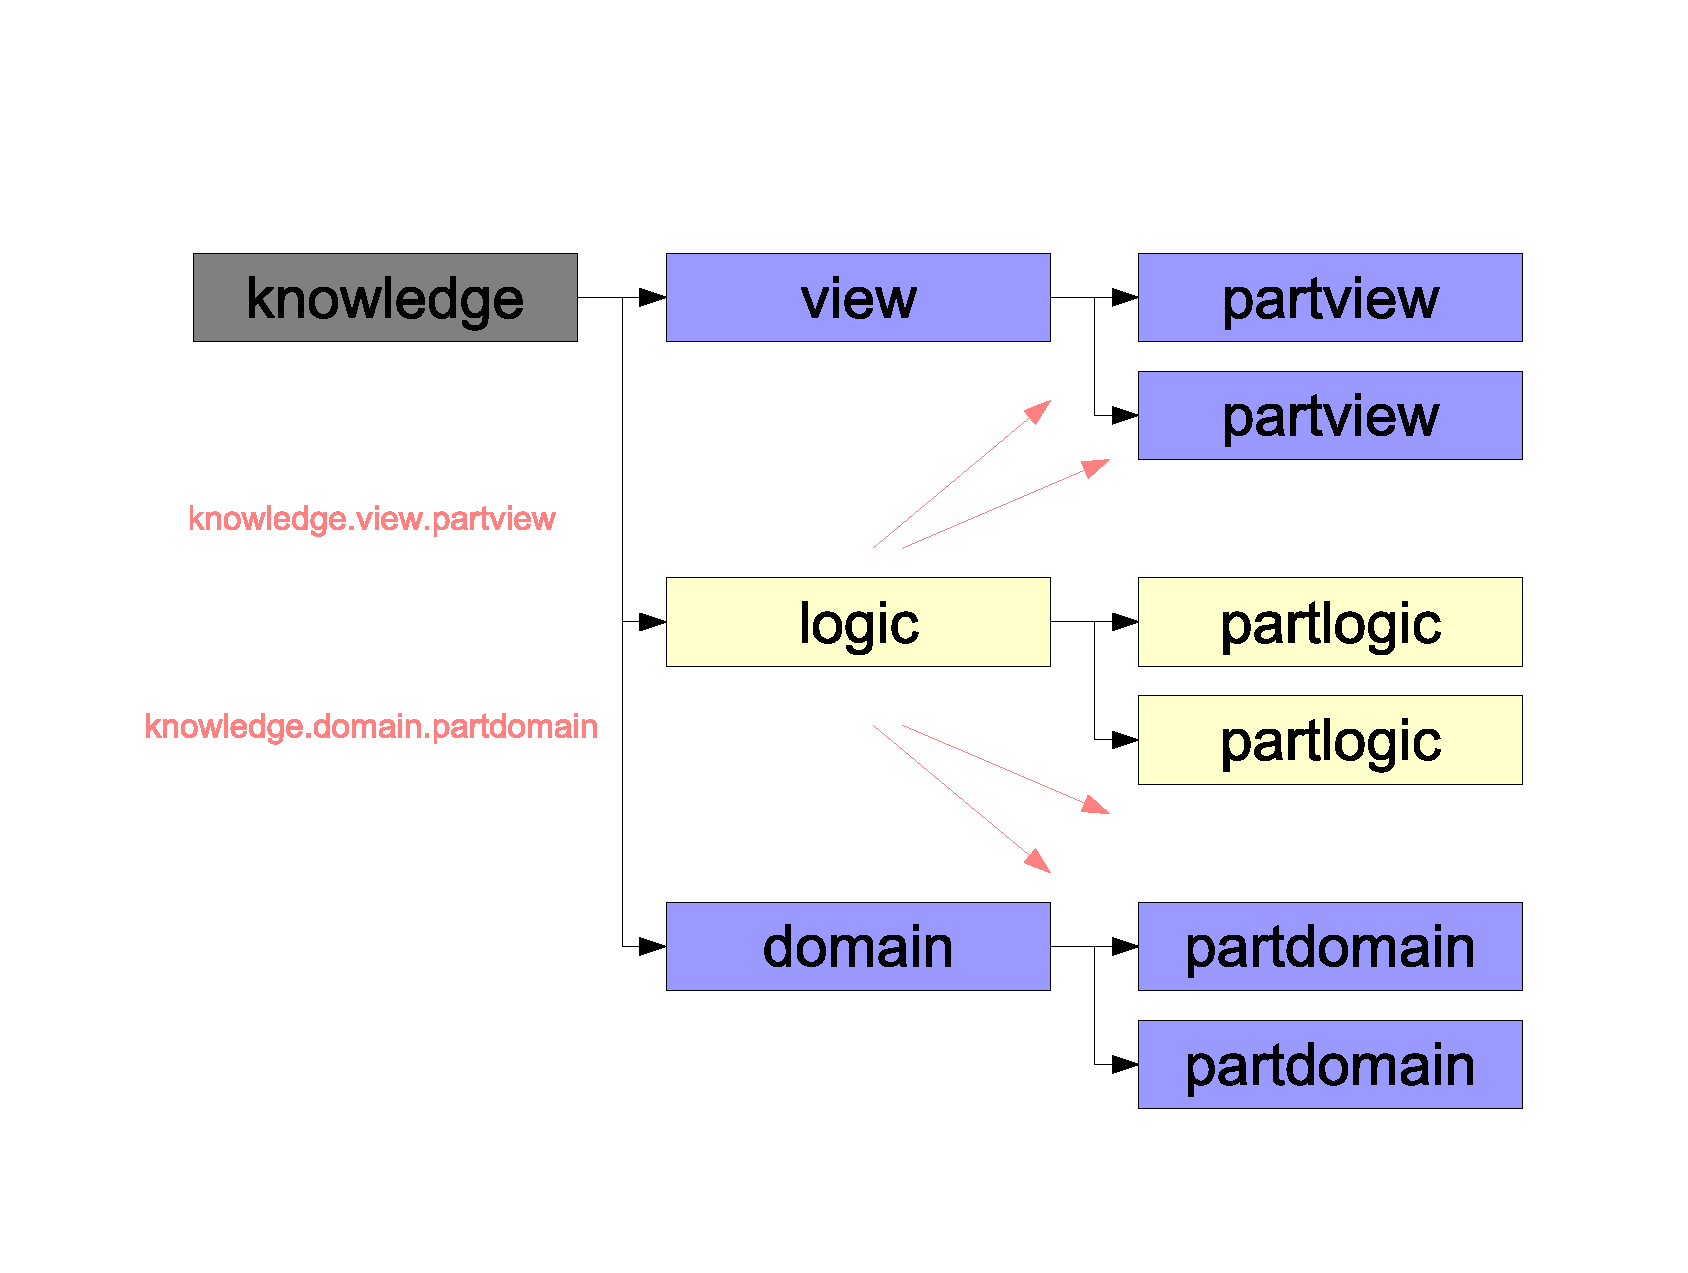
\includegraphics[scale=0.2]{vector/mvctree.eps}
        \caption{Logic manipulating States}
        \label{mvctree_figure}
    \end{center}
\end{figure}

Figure \ref{mvctree_figure} shows the three parts: \emph{Domain} (Model),
\emph{View} and \emph{Logic} (Controller) of an (adapted) MVC pattern as
independent branches of one common knowledge tree, as existent at system
runtime in memory. Each of them represents a concept on its own. The logic
model, however, is allowed to access and change the view- and domain model; it
is able to link different knowledge models. But view- and domain model,
representing states, are not allowed to manipulate logic. In other words: The
dependencies between logic- and state models are \emph{unidirectional}.

An innovation is that logic knowledge gets manipulatable. A logic model
(algorithm) cannot only access and change state-, but also logic models, even
itself! Because models modified in that manner can be made persistent in form
of CYBOL knowledge templates (section \ref{cybol_heading}), and be reloaded the
next time an application starts, this may be seen as a kind of
\emph{Meta Programming}, which \cite{wikipedia} defines as: \textit{the writing
of programs that write or manipulate other programs (or themselves) as their
data.}

The clear separation of states and logic into discrete models avoids unwanted
dependencies as caused by the bundling of attributes and methods in OOP. All
that would be needed to make a CYBOP system work with new state models, is the
corresponding translation logic. Translators \cite{hellerkunze} simplify
architectures and unify communication.

%
% $RCSfile: without_capsules.tex,v $
%
% Copyright (C) 2002-2008. Christian Heller.
%
% Permission is granted to copy, distribute and/or modify this document
% under the terms of the GNU Free Documentation License, Version 1.1 or
% any later version published by the Free Software Foundation; with no
% Invariant Sections, with no Front-Cover Texts and with no Back-Cover
% Texts. A copy of the license is included in the section entitled
% "GNU Free Documentation License".
%
% http://www.cybop.net
% - Cybernetics Oriented Programming -
%
% http://www.resmedicinae.org
% - Information in Medicine -
%
% Version: $Revision: 1.1 $ $Date: 2008-08-19 20:41:09 $ $Author: christian $
% Authors: Christian Heller <christian.heller@tuxtax.de>
%

\subsection{Without Capsules?}
\label{without_capsules_heading}
\index{Without Capsules}
\index{Side Effect}
\index{Knowledge Tree}
\index{Encapsulation}
\index{Well-Defined Knowledge Paths}
\index{Call by Reference}
\index{Call by Value}

Once again it has to be said that all this becomes possible only because all
domain/ application knowledge is stored together in one single tree structure
which is hold and managed by the \emph{Cybernetics Oriented Interpreter}
(CYBOI) (chapter \ref{cybernetics_oriented_interpreter_heading}). What was
traditionally criticised as \emph{Side Effect}, is now a \emph{wanted} effect.
Low-level system procedures within CYBOI forward just one pointer -- the root
of the knowledge tree, which they all may access and manipulate. Data values do
\emph{not} get copied among procedures; they exist just once in the knowledge
tree and may be used by any procedure. Of course, this also means that any
application has access to the knowledge of any other application. Ways ensuring
sufficient security have to be found here (section \ref{future_works_heading}).

Besides the \emph{Encapsulation} of data through \emph{Procedures}, there are
other forms of encapsulating data, such as the \emph{Class} (section
\ref{object_oriented_programming_heading}). One of its purposes was to preserve
transient data in memory, another to restrict access to certain data. In CYBOP,
both tasks are taken care of by CYBOI. It holds the singular knowledge tree and
manages access to it, through well-defined low-level procedures.

There are a number of advantages to this style of programming: An application
developer has no chance of accessing memory areas directly, which prevents
memory leaks and wrong pointers. Because all knowledge can be accessed through
well-defined paths into the knowledge tree only, arbitrary security mechanisms
may be applied and switched as needed, at runtime. Since all algorithms (logic
knowledge) work with references to data in the knowledge tree
(\emph{Call by Reference}), no more data values need to be copied locally
(\emph{Call by Value}), which ensures efficient memory usage. Errors are not to
be expected, because nonexisting knowledge references are simply ignored by
CYBOI.


